% Options for packages loaded elsewhere
\PassOptionsToPackage{unicode}{hyperref}
\PassOptionsToPackage{hyphens}{url}
\PassOptionsToPackage{dvipsnames,svgnames,x11names}{xcolor}
%
\documentclass[
  letterpaper,
  DIV=11,
  numbers=noendperiod]{scrartcl}

\usepackage{amsmath,amssymb}
\usepackage{iftex}
\ifPDFTeX
  \usepackage[T1]{fontenc}
  \usepackage[utf8]{inputenc}
  \usepackage{textcomp} % provide euro and other symbols
\else % if luatex or xetex
  \usepackage{unicode-math}
  \defaultfontfeatures{Scale=MatchLowercase}
  \defaultfontfeatures[\rmfamily]{Ligatures=TeX,Scale=1}
\fi
\usepackage{lmodern}
\ifPDFTeX\else  
    % xetex/luatex font selection
\fi
% Use upquote if available, for straight quotes in verbatim environments
\IfFileExists{upquote.sty}{\usepackage{upquote}}{}
\IfFileExists{microtype.sty}{% use microtype if available
  \usepackage[]{microtype}
  \UseMicrotypeSet[protrusion]{basicmath} % disable protrusion for tt fonts
}{}
\makeatletter
\@ifundefined{KOMAClassName}{% if non-KOMA class
  \IfFileExists{parskip.sty}{%
    \usepackage{parskip}
  }{% else
    \setlength{\parindent}{0pt}
    \setlength{\parskip}{6pt plus 2pt minus 1pt}}
}{% if KOMA class
  \KOMAoptions{parskip=half}}
\makeatother
\usepackage{xcolor}
\setlength{\emergencystretch}{3em} % prevent overfull lines
\setcounter{secnumdepth}{-\maxdimen} % remove section numbering
% Make \paragraph and \subparagraph free-standing
\makeatletter
\ifx\paragraph\undefined\else
  \let\oldparagraph\paragraph
  \renewcommand{\paragraph}{
    \@ifstar
      \xxxParagraphStar
      \xxxParagraphNoStar
  }
  \newcommand{\xxxParagraphStar}[1]{\oldparagraph*{#1}\mbox{}}
  \newcommand{\xxxParagraphNoStar}[1]{\oldparagraph{#1}\mbox{}}
\fi
\ifx\subparagraph\undefined\else
  \let\oldsubparagraph\subparagraph
  \renewcommand{\subparagraph}{
    \@ifstar
      \xxxSubParagraphStar
      \xxxSubParagraphNoStar
  }
  \newcommand{\xxxSubParagraphStar}[1]{\oldsubparagraph*{#1}\mbox{}}
  \newcommand{\xxxSubParagraphNoStar}[1]{\oldsubparagraph{#1}\mbox{}}
\fi
\makeatother

\usepackage{color}
\usepackage{fancyvrb}
\newcommand{\VerbBar}{|}
\newcommand{\VERB}{\Verb[commandchars=\\\{\}]}
\DefineVerbatimEnvironment{Highlighting}{Verbatim}{commandchars=\\\{\}}
% Add ',fontsize=\small' for more characters per line
\usepackage{framed}
\definecolor{shadecolor}{RGB}{241,243,245}
\newenvironment{Shaded}{\begin{snugshade}}{\end{snugshade}}
\newcommand{\AlertTok}[1]{\textcolor[rgb]{0.68,0.00,0.00}{#1}}
\newcommand{\AnnotationTok}[1]{\textcolor[rgb]{0.37,0.37,0.37}{#1}}
\newcommand{\AttributeTok}[1]{\textcolor[rgb]{0.40,0.45,0.13}{#1}}
\newcommand{\BaseNTok}[1]{\textcolor[rgb]{0.68,0.00,0.00}{#1}}
\newcommand{\BuiltInTok}[1]{\textcolor[rgb]{0.00,0.23,0.31}{#1}}
\newcommand{\CharTok}[1]{\textcolor[rgb]{0.13,0.47,0.30}{#1}}
\newcommand{\CommentTok}[1]{\textcolor[rgb]{0.37,0.37,0.37}{#1}}
\newcommand{\CommentVarTok}[1]{\textcolor[rgb]{0.37,0.37,0.37}{\textit{#1}}}
\newcommand{\ConstantTok}[1]{\textcolor[rgb]{0.56,0.35,0.01}{#1}}
\newcommand{\ControlFlowTok}[1]{\textcolor[rgb]{0.00,0.23,0.31}{\textbf{#1}}}
\newcommand{\DataTypeTok}[1]{\textcolor[rgb]{0.68,0.00,0.00}{#1}}
\newcommand{\DecValTok}[1]{\textcolor[rgb]{0.68,0.00,0.00}{#1}}
\newcommand{\DocumentationTok}[1]{\textcolor[rgb]{0.37,0.37,0.37}{\textit{#1}}}
\newcommand{\ErrorTok}[1]{\textcolor[rgb]{0.68,0.00,0.00}{#1}}
\newcommand{\ExtensionTok}[1]{\textcolor[rgb]{0.00,0.23,0.31}{#1}}
\newcommand{\FloatTok}[1]{\textcolor[rgb]{0.68,0.00,0.00}{#1}}
\newcommand{\FunctionTok}[1]{\textcolor[rgb]{0.28,0.35,0.67}{#1}}
\newcommand{\ImportTok}[1]{\textcolor[rgb]{0.00,0.46,0.62}{#1}}
\newcommand{\InformationTok}[1]{\textcolor[rgb]{0.37,0.37,0.37}{#1}}
\newcommand{\KeywordTok}[1]{\textcolor[rgb]{0.00,0.23,0.31}{\textbf{#1}}}
\newcommand{\NormalTok}[1]{\textcolor[rgb]{0.00,0.23,0.31}{#1}}
\newcommand{\OperatorTok}[1]{\textcolor[rgb]{0.37,0.37,0.37}{#1}}
\newcommand{\OtherTok}[1]{\textcolor[rgb]{0.00,0.23,0.31}{#1}}
\newcommand{\PreprocessorTok}[1]{\textcolor[rgb]{0.68,0.00,0.00}{#1}}
\newcommand{\RegionMarkerTok}[1]{\textcolor[rgb]{0.00,0.23,0.31}{#1}}
\newcommand{\SpecialCharTok}[1]{\textcolor[rgb]{0.37,0.37,0.37}{#1}}
\newcommand{\SpecialStringTok}[1]{\textcolor[rgb]{0.13,0.47,0.30}{#1}}
\newcommand{\StringTok}[1]{\textcolor[rgb]{0.13,0.47,0.30}{#1}}
\newcommand{\VariableTok}[1]{\textcolor[rgb]{0.07,0.07,0.07}{#1}}
\newcommand{\VerbatimStringTok}[1]{\textcolor[rgb]{0.13,0.47,0.30}{#1}}
\newcommand{\WarningTok}[1]{\textcolor[rgb]{0.37,0.37,0.37}{\textit{#1}}}

\providecommand{\tightlist}{%
  \setlength{\itemsep}{0pt}\setlength{\parskip}{0pt}}\usepackage{longtable,booktabs,array}
\usepackage{calc} % for calculating minipage widths
% Correct order of tables after \paragraph or \subparagraph
\usepackage{etoolbox}
\makeatletter
\patchcmd\longtable{\par}{\if@noskipsec\mbox{}\fi\par}{}{}
\makeatother
% Allow footnotes in longtable head/foot
\IfFileExists{footnotehyper.sty}{\usepackage{footnotehyper}}{\usepackage{footnote}}
\makesavenoteenv{longtable}
\usepackage{graphicx}
\makeatletter
\def\maxwidth{\ifdim\Gin@nat@width>\linewidth\linewidth\else\Gin@nat@width\fi}
\def\maxheight{\ifdim\Gin@nat@height>\textheight\textheight\else\Gin@nat@height\fi}
\makeatother
% Scale images if necessary, so that they will not overflow the page
% margins by default, and it is still possible to overwrite the defaults
% using explicit options in \includegraphics[width, height, ...]{}
\setkeys{Gin}{width=\maxwidth,height=\maxheight,keepaspectratio}
% Set default figure placement to htbp
\makeatletter
\def\fps@figure{htbp}
\makeatother

\KOMAoption{captions}{tableheading}
\makeatletter
\@ifpackageloaded{caption}{}{\usepackage{caption}}
\AtBeginDocument{%
\ifdefined\contentsname
  \renewcommand*\contentsname{Table of contents}
\else
  \newcommand\contentsname{Table of contents}
\fi
\ifdefined\listfigurename
  \renewcommand*\listfigurename{List of Figures}
\else
  \newcommand\listfigurename{List of Figures}
\fi
\ifdefined\listtablename
  \renewcommand*\listtablename{List of Tables}
\else
  \newcommand\listtablename{List of Tables}
\fi
\ifdefined\figurename
  \renewcommand*\figurename{Figure}
\else
  \newcommand\figurename{Figure}
\fi
\ifdefined\tablename
  \renewcommand*\tablename{Table}
\else
  \newcommand\tablename{Table}
\fi
}
\@ifpackageloaded{float}{}{\usepackage{float}}
\floatstyle{ruled}
\@ifundefined{c@chapter}{\newfloat{codelisting}{h}{lop}}{\newfloat{codelisting}{h}{lop}[chapter]}
\floatname{codelisting}{Listing}
\newcommand*\listoflistings{\listof{codelisting}{List of Listings}}
\makeatother
\makeatletter
\makeatother
\makeatletter
\@ifpackageloaded{caption}{}{\usepackage{caption}}
\@ifpackageloaded{subcaption}{}{\usepackage{subcaption}}
\makeatother
\makeatletter
\@ifpackageloaded{tikz}{}{\usepackage{tikz}}
\makeatother
        \newcommand*\circled[1]{\tikz[baseline=(char.base)]{
          \node[shape=circle,draw,inner sep=1pt] (char) {{\scriptsize#1}};}}  
                  

\ifLuaTeX
  \usepackage{selnolig}  % disable illegal ligatures
\fi
\usepackage{bookmark}

\IfFileExists{xurl.sty}{\usepackage{xurl}}{} % add URL line breaks if available
\urlstyle{same} % disable monospaced font for URLs
\hypersetup{
  pdftitle={week 2: linear model and causal inference},
  colorlinks=true,
  linkcolor={blue},
  filecolor={Maroon},
  citecolor={Blue},
  urlcolor={Blue},
  pdfcreator={LaTeX via pandoc}}


\title{week 2: linear model and causal inference}
\usepackage{etoolbox}
\makeatletter
\providecommand{\subtitle}[1]{% add subtitle to \maketitle
  \apptocmd{\@title}{\par {\large #1 \par}}{}{}
}
\makeatother
\subtitle{geocentric models}
\author{}
\date{}

\begin{document}
\maketitle


\subsubsection{Annoucements and such}\label{annoucements-and-such}

\begin{itemize}
\tightlist
\item
  We will start using \texttt{brms} today! Install this package now, if
  you haven't already.
\end{itemize}

\begin{Shaded}
\begin{Highlighting}[]
\FunctionTok{install.packages}\NormalTok{(}\FunctionTok{c}\NormalTok{(}\StringTok{"brms"}\NormalTok{,}\StringTok{"tidybayes"}\NormalTok{))}
\end{Highlighting}
\end{Shaded}

\begin{itemize}
\tightlist
\item
  No office hours Friday
\item
  \href{https://hr.uoregon.edu/outstanding-employee-awards}{Lori Olsen}
\item
  Projects
\end{itemize}

\subsubsection{Workspace setup}\label{workspace-setup}

\begin{Shaded}
\begin{Highlighting}[]
\FunctionTok{library}\NormalTok{(here)}
\FunctionTok{library}\NormalTok{(tidyverse)}
\FunctionTok{library}\NormalTok{(cowplot)}
\FunctionTok{library}\NormalTok{(brms)}
\FunctionTok{library}\NormalTok{(tidybayes)}
\FunctionTok{library}\NormalTok{(patchwork)}
\end{Highlighting}
\end{Shaded}

\begin{center}\rule{0.5\linewidth}{0.5pt}\end{center}

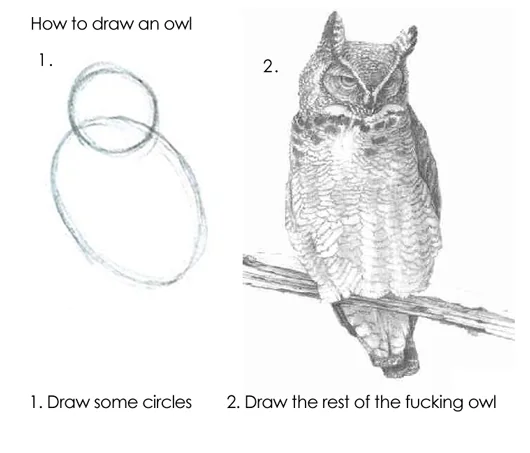
\includegraphics{images/2-1_owl.png}

\subsubsection{Workflow}\label{workflow}

\begin{enumerate}
\def\labelenumi{\arabic{enumi}.}
\item
  State a clear question.
\item
  Sketch your causal assumptions.
\item
  Use the sketch to define a generative model.
\item
  Use the generative model to build an estimator.
\item
  Profit.
\end{enumerate}

\begin{center}\rule{0.5\linewidth}{0.5pt}\end{center}

\subsection{Model ``recipes''}\label{model-recipes}

\begin{enumerate}
\def\labelenumi{\arabic{enumi}.}
\tightlist
\item
  Recognize a set of variables to work with. (Data and parameters.)
\item
  Define each variable either in terms of the other variables OR in
  terms of a probability distribution.
\item
  The combination of variables and their probability distributions
  defines a \textbf{joint generative model} that can be used to simulate
  hypothetical observations and analyze real ones.
\end{enumerate}

Here's an example:

\begin{align*}
y_i &\sim \text{Normal}(\mu_i,\sigma) \\
\mu_i &= \beta x_i \\
\beta &\sim \text{Normal}(0,10) \\
\sigma &\sim \text{Exponential}(1) \\
x_i &\sim \text{Normal}(0,1) \\
\end{align*}

\begin{center}\rule{0.5\linewidth}{0.5pt}\end{center}

\subsubsection{Model for globe-tossing}\label{model-for-globe-tossing}

Here's the model for last week's globe-tossing experiment:

\begin{align*}
W &\sim \text{Binomial}(N,p) \\
p &\sim \text{Uniform}(0,1) \\
\end{align*}

\begin{itemize}
\tightlist
\item
  \(W\) is the observed count of water.
\item
  \(N\) is the total number of tosses.
\item
  \(p\) is the proportion of water on the globe.
\end{itemize}

The whole model can be read as:

\begin{quote}
The count \(W\) is distributed binomially with sample size \(N\) and
probability \(p\). The prior for \(p\) is assumed to be uniform between
0 and 1.
\end{quote}

\begin{center}\rule{0.5\linewidth}{0.5pt}\end{center}

\subsubsection{Model for globe-tossing}\label{model-for-globe-tossing-1}

Here's the model for last week's globe-tossing experiment:

\begin{align*}
W &\sim \text{Binomial}(N,p) \\
p &\sim \text{Uniform}(0,1) \\
\end{align*}

\paragraph{\texorpdfstring{Estimating the posterior using
\texttt{brms}}{Estimating the posterior using brms}}\label{estimating-the-posterior-using-brms}

Last week, we used grid approximation to estimate the posterior
distribution. In the video you watched for today, McElreath moves on to
something called \textbf{QUADRATIC APPROXIMATION}. It's good to
understand what that's doing, but you and I are moving right along to
MCMC. We won't go into the details of what's happening for a few weeks,
but let's start with the code to estimate the model.

Let's say we tossed the globe 9 times and observed 6 waters:

\phantomsection\label{annotated-cell-3}%
\begin{Shaded}
\begin{Highlighting}[]
\NormalTok{m1 }\OtherTok{\textless{}{-}}
  \FunctionTok{brm}\NormalTok{(}\AttributeTok{data =} \FunctionTok{list}\NormalTok{(}\AttributeTok{w =} \DecValTok{6}\NormalTok{), }\hspace*{\fill}\NormalTok{\circled{1}}
      \AttributeTok{family =} \FunctionTok{binomial}\NormalTok{(}\AttributeTok{link =} \StringTok{"identity"}\NormalTok{), }\hspace*{\fill}\NormalTok{\circled{2}}
\NormalTok{      w }\SpecialCharTok{|} \FunctionTok{trials}\NormalTok{(}\DecValTok{9}\NormalTok{) }\SpecialCharTok{\textasciitilde{}} \DecValTok{0} \SpecialCharTok{+}\NormalTok{ Intercept, }\hspace*{\fill}\NormalTok{\circled{3}}
      \FunctionTok{prior}\NormalTok{(}\FunctionTok{uniform}\NormalTok{(}\DecValTok{0}\NormalTok{, }\DecValTok{1}\NormalTok{), }\AttributeTok{class =}\NormalTok{ b), }\hspace*{\fill}\NormalTok{\circled{4}}
      \AttributeTok{iter =} \DecValTok{5000}\NormalTok{, }\AttributeTok{warmup =} \DecValTok{1000}\NormalTok{, }\AttributeTok{seed =} \DecValTok{3}\NormalTok{, }\AttributeTok{chains=}\DecValTok{1}\NormalTok{, }\hspace*{\fill}\NormalTok{\circled{5}}
      \AttributeTok{file =} \FunctionTok{here}\NormalTok{(}\StringTok{"files/models/m21.1"}\NormalTok{)) }\hspace*{\fill}\NormalTok{\circled{6}}
\end{Highlighting}
\end{Shaded}

\begin{description}
\tightlist
\item[\circled{1}]
Data can be a data frame or a list. Just make sure the variable names
match what's in your formula.
\item[\circled{2}]
How you assume your \textbf{outcome} variable is distributed.
\item[\circled{3}]
The formula for your outcome.
\item[\circled{4}]
Priors for \emph{every} parameter in your model. Here, we only have one
parameter, so we only need 1 prior. This happens to be a flat prior
between 0 and 1.
\item[\circled{5}]
Some choices about how we want our model to run. We'll go more into this
later.
\item[\circled{6}]
These models can take a long time to run. You can automatically save the
output to a file; when you do this, the next time you run this code, it
won't actually estimate the model, but will instead pull the output from
your stated file. Be WARNED: if you change the data or the model code,
it will NOT restimate your model until you delete the file.
\end{description}

\begin{center}\rule{0.5\linewidth}{0.5pt}\end{center}

\subsubsection{Sampling from the
posterior}\label{sampling-from-the-posterior}

Grid approximation gave us the calculated probability of each possible
value of our parameter, \(p\). But our method of conducting bayes will
no longer give us such a neat solution. Here's how you get the posterior
distribution for \(p\):

\begin{Shaded}
\begin{Highlighting}[]
\NormalTok{samples\_from\_post }\OtherTok{=} \FunctionTok{as\_draws\_df}\NormalTok{(m1)}
\NormalTok{samples\_from\_post}
\end{Highlighting}
\end{Shaded}

\begin{verbatim}
# A draws_df: 4000 iterations, 1 chains, and 3 variables
   b_Intercept lprior lp__
1         0.46      0 -2.1
2         0.49      0 -1.9
3         0.56      0 -1.5
4         0.66      0 -1.3
5         0.71      0 -1.3
6         0.62      0 -1.3
7         0.68      0 -1.3
8         0.55      0 -1.5
9         0.63      0 -1.3
10        0.67      0 -1.3
# ... with 3990 more draws
# ... hidden reserved variables {'.chain', '.iteration', '.draw'}
\end{verbatim}

\begin{center}\rule{0.5\linewidth}{0.5pt}\end{center}

\begin{Shaded}
\begin{Highlighting}[]
\NormalTok{samples\_from\_post }\SpecialCharTok{\%\textgreater{}\%}  
  \FunctionTok{ggplot}\NormalTok{(}\FunctionTok{aes}\NormalTok{(}\AttributeTok{x=}\NormalTok{b\_Intercept)) }\SpecialCharTok{+}
  \FunctionTok{geom\_density}\NormalTok{(}\AttributeTok{fill =} \StringTok{"grey"}\NormalTok{, }\AttributeTok{color =} \StringTok{"white"}\NormalTok{) }\SpecialCharTok{+}
  \FunctionTok{labs}\NormalTok{(}\AttributeTok{x=}\StringTok{"Proportion water"}\NormalTok{)}
\end{Highlighting}
\end{Shaded}

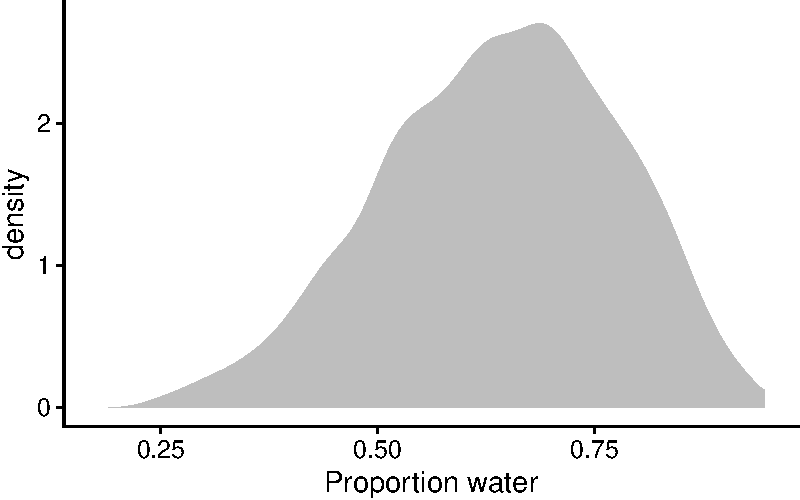
\includegraphics[width=17.1875in,height=\textheight]{lecture02-1_files/figure-pdf/unnamed-chunk-6-1.pdf}

\begin{center}\rule{0.5\linewidth}{0.5pt}\end{center}

\subsubsection{Posterior predictive
distribution}\label{posterior-predictive-distribution}

\begin{Shaded}
\begin{Highlighting}[]
\NormalTok{ppd }\OtherTok{=} \FunctionTok{posterior\_predict}\NormalTok{(m1)}
\FunctionTok{dim}\NormalTok{(ppd)}
\end{Highlighting}
\end{Shaded}

\begin{verbatim}
[1] 4000    1
\end{verbatim}

\begin{Shaded}
\begin{Highlighting}[]
\NormalTok{ppd}
\end{Highlighting}
\end{Shaded}

\begin{verbatim}
        [,1]
   [1,]    3
   [2,]    5
   [3,]    7
   [4,]    6
   [5,]    5
   [6,]    5
   [7,]    7
   [8,]    4
   [9,]    4
  [10,]    7
  [11,]    7
  [12,]    5
  [13,]    8
  [14,]    8
  [15,]    8
  [16,]    6
  [17,]    6
  [18,]    8
  [19,]    9
  [20,]    9
  [21,]    8
  [22,]    8
  [23,]    3
  [24,]    7
  [25,]    6
  [26,]    5
  [27,]    7
  [28,]    5
  [29,]    7
  [30,]    5
  [31,]    8
  [32,]    7
  [33,]    5
  [34,]    6
  [35,]    4
  [36,]    4
  [37,]    6
  [38,]    8
  [39,]    4
  [40,]    5
  [41,]    6
  [42,]    8
  [43,]    8
  [44,]    8
  [45,]    5
  [46,]    6
  [47,]    8
  [48,]    4
  [49,]    6
  [50,]    6
  [51,]    7
  [52,]    4
  [53,]    6
  [54,]    7
  [55,]    6
  [56,]    6
  [57,]    5
  [58,]    4
  [59,]    3
  [60,]    6
  [61,]    5
  [62,]    5
  [63,]    5
  [64,]    7
  [65,]    8
  [66,]    5
  [67,]    8
  [68,]    8
  [69,]    5
  [70,]    9
  [71,]    8
  [72,]    3
  [73,]    8
  [74,]    7
  [75,]    8
  [76,]    4
  [77,]    4
  [78,]    4
  [79,]    7
  [80,]    4
  [81,]    8
  [82,]    4
  [83,]    6
  [84,]    6
  [85,]    6
  [86,]    7
  [87,]    5
  [88,]    7
  [89,]    7
  [90,]    8
  [91,]    7
  [92,]    2
  [93,]    2
  [94,]    3
  [95,]    5
  [96,]    9
  [97,]    5
  [98,]    6
  [99,]    6
 [100,]    7
 [101,]    5
 [102,]    7
 [103,]    5
 [104,]    6
 [105,]    6
 [106,]    8
 [107,]    7
 [108,]    8
 [109,]    5
 [110,]    8
 [111,]    3
 [112,]    6
 [113,]    6
 [114,]    8
 [115,]    2
 [116,]    7
 [117,]    8
 [118,]    5
 [119,]    7
 [120,]    7
 [121,]    7
 [122,]    7
 [123,]    6
 [124,]    6
 [125,]    8
 [126,]    8
 [127,]    6
 [128,]    5
 [129,]    7
 [130,]    7
 [131,]    6
 [132,]    8
 [133,]    7
 [134,]    6
 [135,]    5
 [136,]    6
 [137,]    5
 [138,]    6
 [139,]    8
 [140,]    6
 [141,]    5
 [142,]    8
 [143,]    6
 [144,]    6
 [145,]    6
 [146,]    8
 [147,]    7
 [148,]    5
 [149,]    5
 [150,]    4
 [151,]    6
 [152,]    9
 [153,]    8
 [154,]    8
 [155,]    6
 [156,]    6
 [157,]    4
 [158,]    6
 [159,]    5
 [160,]    3
 [161,]    6
 [162,]    7
 [163,]    7
 [164,]    9
 [165,]    4
 [166,]    5
 [167,]    6
 [168,]    4
 [169,]    4
 [170,]    4
 [171,]    7
 [172,]    4
 [173,]    9
 [174,]    7
 [175,]    7
 [176,]    6
 [177,]    7
 [178,]    7
 [179,]    8
 [180,]    7
 [181,]    3
 [182,]    8
 [183,]    9
 [184,]    7
 [185,]    8
 [186,]    5
 [187,]    7
 [188,]    7
 [189,]    5
 [190,]    2
 [191,]    6
 [192,]    9
 [193,]    6
 [194,]    5
 [195,]    8
 [196,]    4
 [197,]    2
 [198,]    4
 [199,]    6
 [200,]    8
 [201,]    8
 [202,]    7
 [203,]    8
 [204,]    9
 [205,]    3
 [206,]    4
 [207,]    7
 [208,]    8
 [209,]    5
 [210,]    7
 [211,]    7
 [212,]    4
 [213,]    7
 [214,]    6
 [215,]    9
 [216,]    8
 [217,]    9
 [218,]    8
 [219,]    5
 [220,]    6
 [221,]    6
 [222,]    3
 [223,]    4
 [224,]    7
 [225,]    8
 [226,]    6
 [227,]    4
 [228,]    8
 [229,]    7
 [230,]    5
 [231,]    7
 [232,]    6
 [233,]    7
 [234,]    7
 [235,]    1
 [236,]    5
 [237,]    8
 [238,]    6
 [239,]    7
 [240,]    2
 [241,]    4
 [242,]    8
 [243,]    9
 [244,]    9
 [245,]    5
 [246,]    7
 [247,]    5
 [248,]    7
 [249,]    5
 [250,]    4
 [251,]    7
 [252,]    8
 [253,]    7
 [254,]    5
 [255,]    6
 [256,]    9
 [257,]    6
 [258,]    7
 [259,]    4
 [260,]    6
 [261,]    6
 [262,]    6
 [263,]    7
 [264,]    3
 [265,]    6
 [266,]    5
 [267,]    4
 [268,]    6
 [269,]    8
 [270,]    5
 [271,]    2
 [272,]    5
 [273,]    7
 [274,]    7
 [275,]    4
 [276,]    6
 [277,]    7
 [278,]    9
 [279,]    8
 [280,]    6
 [281,]    6
 [282,]    4
 [283,]    4
 [284,]    5
 [285,]    5
 [286,]    5
 [287,]    4
 [288,]    9
 [289,]    9
 [290,]    8
 [291,]    8
 [292,]    8
 [293,]    8
 [294,]    2
 [295,]    5
 [296,]    6
 [297,]    9
 [298,]    6
 [299,]    5
 [300,]    3
 [301,]    5
 [302,]    7
 [303,]    4
 [304,]    5
 [305,]    8
 [306,]    9
 [307,]    7
 [308,]    4
 [309,]    6
 [310,]    8
 [311,]    4
 [312,]    8
 [313,]    6
 [314,]    8
 [315,]    5
 [316,]    6
 [317,]    9
 [318,]    8
 [319,]    9
 [320,]    7
 [321,]    9
 [322,]    2
 [323,]    4
 [324,]    3
 [325,]    5
 [326,]    7
 [327,]    6
 [328,]    6
 [329,]    5
 [330,]    5
 [331,]    5
 [332,]    8
 [333,]    6
 [334,]    6
 [335,]    7
 [336,]    9
 [337,]    9
 [338,]    4
 [339,]    1
 [340,]    2
 [341,]    6
 [342,]    4
 [343,]    6
 [344,]    8
 [345,]    5
 [346,]    7
 [347,]    7
 [348,]    7
 [349,]    8
 [350,]    7
 [351,]    6
 [352,]    6
 [353,]    3
 [354,]    7
 [355,]    4
 [356,]    4
 [357,]    7
 [358,]    3
 [359,]    2
 [360,]    5
 [361,]    5
 [362,]    5
 [363,]    7
 [364,]    6
 [365,]    7
 [366,]    6
 [367,]    4
 [368,]    2
 [369,]    8
 [370,]    8
 [371,]    3
 [372,]    1
 [373,]    4
 [374,]    4
 [375,]    2
 [376,]    3
 [377,]    4
 [378,]    4
 [379,]    5
 [380,]    4
 [381,]    5
 [382,]    8
 [383,]    6
 [384,]    8
 [385,]    5
 [386,]    7
 [387,]    8
 [388,]    6
 [389,]    4
 [390,]    5
 [391,]    6
 [392,]    7
 [393,]    6
 [394,]    5
 [395,]    6
 [396,]    6
 [397,]    6
 [398,]    8
 [399,]    9
 [400,]    7
 [401,]    7
 [402,]    6
 [403,]    7
 [404,]    3
 [405,]    4
 [406,]    8
 [407,]    6
 [408,]    7
 [409,]    8
 [410,]    7
 [411,]    6
 [412,]    7
 [413,]    4
 [414,]    5
 [415,]    5
 [416,]    6
 [417,]    6
 [418,]    5
 [419,]    5
 [420,]    4
 [421,]    6
 [422,]    4
 [423,]    7
 [424,]    5
 [425,]    7
 [426,]    6
 [427,]    1
 [428,]    9
 [429,]    6
 [430,]    7
 [431,]    7
 [432,]    4
 [433,]    2
 [434,]    6
 [435,]    8
 [436,]    7
 [437,]    7
 [438,]    5
 [439,]    6
 [440,]    8
 [441,]    7
 [442,]    6
 [443,]    6
 [444,]    7
 [445,]    2
 [446,]    3
 [447,]    6
 [448,]    8
 [449,]    6
 [450,]    5
 [451,]    4
 [452,]    4
 [453,]    8
 [454,]    6
 [455,]    6
 [456,]    4
 [457,]    8
 [458,]    8
 [459,]    6
 [460,]    4
 [461,]    6
 [462,]    8
 [463,]    8
 [464,]    7
 [465,]    7
 [466,]    5
 [467,]    7
 [468,]    4
 [469,]    7
 [470,]    5
 [471,]    4
 [472,]    8
 [473,]    6
 [474,]    6
 [475,]    7
 [476,]    6
 [477,]    4
 [478,]    4
 [479,]    7
 [480,]    6
 [481,]    5
 [482,]    3
 [483,]    4
 [484,]    4
 [485,]    4
 [486,]    7
 [487,]    5
 [488,]    6
 [489,]    5
 [490,]    4
 [491,]    8
 [492,]    7
 [493,]    4
 [494,]    7
 [495,]    8
 [496,]    4
 [497,]    8
 [498,]    4
 [499,]    8
 [500,]    6
 [501,]    3
 [502,]    5
 [503,]    5
 [504,]    5
 [505,]    6
 [506,]    7
 [507,]    6
 [508,]    8
 [509,]    6
 [510,]    5
 [511,]    6
 [512,]    5
 [513,]    9
 [514,]    7
 [515,]    4
 [516,]    6
 [517,]    6
 [518,]    7
 [519,]    7
 [520,]    4
 [521,]    1
 [522,]    3
 [523,]    3
 [524,]    4
 [525,]    4
 [526,]    7
 [527,]    7
 [528,]    6
 [529,]    6
 [530,]    6
 [531,]    7
 [532,]    8
 [533,]    5
 [534,]    7
 [535,]    6
 [536,]    2
 [537,]    6
 [538,]    6
 [539,]    6
 [540,]    5
 [541,]    6
 [542,]    5
 [543,]    5
 [544,]    6
 [545,]    6
 [546,]    6
 [547,]    7
 [548,]    5
 [549,]    8
 [550,]    7
 [551,]    9
 [552,]    9
 [553,]    4
 [554,]    6
 [555,]    4
 [556,]    3
 [557,]    1
 [558,]    5
 [559,]    4
 [560,]    7
 [561,]    6
 [562,]    7
 [563,]    7
 [564,]    8
 [565,]    6
 [566,]    5
 [567,]    1
 [568,]    6
 [569,]    8
 [570,]    7
 [571,]    5
 [572,]    3
 [573,]    4
 [574,]    3
 [575,]    6
 [576,]    7
 [577,]    7
 [578,]    6
 [579,]    9
 [580,]    7
 [581,]    5
 [582,]    7
 [583,]    4
 [584,]    9
 [585,]    4
 [586,]    1
 [587,]    1
 [588,]    2
 [589,]    3
 [590,]    3
 [591,]    8
 [592,]    6
 [593,]    2
 [594,]    4
 [595,]    7
 [596,]    8
 [597,]    5
 [598,]    3
 [599,]    6
 [600,]    6
 [601,]    2
 [602,]    6
 [603,]    4
 [604,]    9
 [605,]    7
 [606,]    8
 [607,]    7
 [608,]    6
 [609,]    5
 [610,]    7
 [611,]    4
 [612,]    4
 [613,]    8
 [614,]    6
 [615,]    5
 [616,]    5
 [617,]    7
 [618,]    7
 [619,]    7
 [620,]    6
 [621,]    6
 [622,]    7
 [623,]    5
 [624,]    8
 [625,]    3
 [626,]    5
 [627,]    5
 [628,]    6
 [629,]    8
 [630,]    5
 [631,]    6
 [632,]    4
 [633,]    7
 [634,]    6
 [635,]    4
 [636,]    5
 [637,]    7
 [638,]    5
 [639,]    3
 [640,]    2
 [641,]    5
 [642,]    6
 [643,]    7
 [644,]    6
 [645,]    8
 [646,]    8
 [647,]    5
 [648,]    2
 [649,]    4
 [650,]    6
 [651,]    9
 [652,]    7
 [653,]    7
 [654,]    5
 [655,]    6
 [656,]    8
 [657,]    8
 [658,]    7
 [659,]    7
 [660,]    7
 [661,]    6
 [662,]    3
 [663,]    2
 [664,]    1
 [665,]    7
 [666,]    6
 [667,]    8
 [668,]    5
 [669,]    6
 [670,]    5
 [671,]    6
 [672,]    7
 [673,]    3
 [674,]    5
 [675,]    7
 [676,]    6
 [677,]    5
 [678,]    4
 [679,]    9
 [680,]    6
 [681,]    4
 [682,]    5
 [683,]    6
 [684,]    8
 [685,]    8
 [686,]    7
 [687,]    6
 [688,]    4
 [689,]    7
 [690,]    7
 [691,]    7
 [692,]    5
 [693,]    3
 [694,]    5
 [695,]    4
 [696,]    5
 [697,]    5
 [698,]    2
 [699,]    4
 [700,]    4
 [701,]    5
 [702,]    7
 [703,]    7
 [704,]    7
 [705,]    2
 [706,]    6
 [707,]    5
 [708,]    7
 [709,]    7
 [710,]    7
 [711,]    6
 [712,]    6
 [713,]    6
 [714,]    6
 [715,]    8
 [716,]    7
 [717,]    9
 [718,]    7
 [719,]    7
 [720,]    5
 [721,]    4
 [722,]    4
 [723,]    5
 [724,]    5
 [725,]    7
 [726,]    5
 [727,]    6
 [728,]    5
 [729,]    3
 [730,]    4
 [731,]    5
 [732,]    7
 [733,]    4
 [734,]    6
 [735,]    9
 [736,]    6
 [737,]    5
 [738,]    3
 [739,]    7
 [740,]    8
 [741,]    5
 [742,]    6
 [743,]    5
 [744,]    5
 [745,]    6
 [746,]    6
 [747,]    8
 [748,]    3
 [749,]    5
 [750,]    7
 [751,]    5
 [752,]    5
 [753,]    5
 [754,]    7
 [755,]    9
 [756,]    7
 [757,]    5
 [758,]    7
 [759,]    8
 [760,]    5
 [761,]    7
 [762,]    7
 [763,]    5
 [764,]    4
 [765,]    8
 [766,]    8
 [767,]    8
 [768,]    7
 [769,]    5
 [770,]    6
 [771,]    6
 [772,]    2
 [773,]    7
 [774,]    4
 [775,]    5
 [776,]    9
 [777,]    5
 [778,]    5
 [779,]    2
 [780,]    7
 [781,]    6
 [782,]    6
 [783,]    4
 [784,]    1
 [785,]    0
 [786,]    3
 [787,]    4
 [788,]    7
 [789,]    6
 [790,]    9
 [791,]    8
 [792,]    9
 [793,]    7
 [794,]    7
 [795,]    2
 [796,]    4
 [797,]    5
 [798,]    6
 [799,]    8
 [800,]    9
 [801,]    6
 [802,]    9
 [803,]    9
 [804,]    5
 [805,]    8
 [806,]    5
 [807,]    4
 [808,]    9
 [809,]    6
 [810,]    6
 [811,]    6
 [812,]    3
 [813,]    5
 [814,]    6
 [815,]    5
 [816,]    4
 [817,]    6
 [818,]    7
 [819,]    3
 [820,]    6
 [821,]    5
 [822,]    3
 [823,]    4
 [824,]    8
 [825,]    4
 [826,]    2
 [827,]    6
 [828,]    4
 [829,]    4
 [830,]    9
 [831,]    8
 [832,]    7
 [833,]    8
 [834,]    4
 [835,]    4
 [836,]    3
 [837,]    4
 [838,]    4
 [839,]    8
 [840,]    2
 [841,]    6
 [842,]    9
 [843,]    6
 [844,]    8
 [845,]    6
 [846,]    3
 [847,]    7
 [848,]    4
 [849,]    2
 [850,]    4
 [851,]    6
 [852,]    6
 [853,]    7
 [854,]    5
 [855,]    7
 [856,]    5
 [857,]    6
 [858,]    5
 [859,]    7
 [860,]    9
 [861,]    6
 [862,]    6
 [863,]    9
 [864,]    7
 [865,]    7
 [866,]    9
 [867,]    8
 [868,]    6
 [869,]    7
 [870,]    7
 [871,]    3
 [872,]    6
 [873,]    9
 [874,]    6
 [875,]    1
 [876,]    2
 [877,]    4
 [878,]    2
 [879,]    3
 [880,]    3
 [881,]    2
 [882,]    9
 [883,]    9
 [884,]    6
 [885,]    2
 [886,]    6
 [887,]    4
 [888,]    6
 [889,]    5
 [890,]    6
 [891,]    4
 [892,]    5
 [893,]    6
 [894,]    5
 [895,]    5
 [896,]    3
 [897,]    6
 [898,]    8
 [899,]    8
 [900,]    6
 [901,]    7
 [902,]    7
 [903,]    5
 [904,]    5
 [905,]    7
 [906,]    6
 [907,]    6
 [908,]    7
 [909,]    9
 [910,]    9
 [911,]    9
 [912,]    6
 [913,]    6
 [914,]    8
 [915,]    6
 [916,]    7
 [917,]    3
 [918,]    5
 [919,]    6
 [920,]    7
 [921,]    6
 [922,]    4
 [923,]    2
 [924,]    8
 [925,]    6
 [926,]    7
 [927,]    5
 [928,]    8
 [929,]    5
 [930,]    5
 [931,]    4
 [932,]    6
 [933,]    7
 [934,]    5
 [935,]    3
 [936,]    5
 [937,]    5
 [938,]    6
 [939,]    7
 [940,]    9
 [941,]    3
 [942,]    5
 [943,]    6
 [944,]    7
 [945,]    4
 [946,]    6
 [947,]    4
 [948,]    6
 [949,]    5
 [950,]    4
 [951,]    6
 [952,]    5
 [953,]    5
 [954,]    2
 [955,]    2
 [956,]    2
 [957,]    6
 [958,]    9
 [959,]    9
 [960,]    7
 [961,]    6
 [962,]    5
 [963,]    7
 [964,]    5
 [965,]    5
 [966,]    7
 [967,]    4
 [968,]    6
 [969,]    2
 [970,]    5
 [971,]    4
 [972,]    7
 [973,]    3
 [974,]    7
 [975,]    6
 [976,]    7
 [977,]    5
 [978,]    8
 [979,]    6
 [980,]    8
 [981,]    5
 [982,]    6
 [983,]    2
 [984,]    4
 [985,]    5
 [986,]    8
 [987,]    6
 [988,]    4
 [989,]    3
 [990,]    5
 [991,]    5
 [992,]    7
 [993,]    8
 [994,]    3
 [995,]    8
 [996,]    6
 [997,]    6
 [998,]    2
 [999,]    4
[1000,]    2
[1001,]    5
[1002,]    5
[1003,]    8
[1004,]    8
[1005,]    4
[1006,]    8
[1007,]    6
[1008,]    8
[1009,]    8
[1010,]    6
[1011,]    6
[1012,]    6
[1013,]    4
[1014,]    7
[1015,]    7
[1016,]    6
[1017,]    5
[1018,]    9
[1019,]    7
[1020,]    6
[1021,]    2
[1022,]    2
[1023,]    5
[1024,]    6
[1025,]    3
[1026,]    7
[1027,]    7
[1028,]    7
[1029,]    3
[1030,]    7
[1031,]    6
[1032,]    8
[1033,]    7
[1034,]    6
[1035,]    3
[1036,]    6
[1037,]    6
[1038,]    7
[1039,]    5
[1040,]    6
[1041,]    2
[1042,]    3
[1043,]    2
[1044,]    9
[1045,]    6
[1046,]    9
[1047,]    6
[1048,]    5
[1049,]    4
[1050,]    9
[1051,]    7
[1052,]    5
[1053,]    4
[1054,]    7
[1055,]    9
[1056,]    5
[1057,]    4
[1058,]    5
[1059,]    6
[1060,]    6
[1061,]    7
[1062,]    9
[1063,]    8
[1064,]    9
[1065,]    6
[1066,]    6
[1067,]    5
[1068,]    8
[1069,]    6
[1070,]    7
[1071,]    6
[1072,]    7
[1073,]    9
[1074,]    6
[1075,]    6
[1076,]    9
[1077,]    9
[1078,]    6
[1079,]    4
[1080,]    5
[1081,]    6
[1082,]    8
[1083,]    4
[1084,]    7
[1085,]    7
[1086,]    5
[1087,]    7
[1088,]    5
[1089,]    9
[1090,]    4
[1091,]    6
[1092,]    6
[1093,]    7
[1094,]    7
[1095,]    6
[1096,]    6
[1097,]    5
[1098,]    5
[1099,]    4
[1100,]    4
[1101,]    6
[1102,]    6
[1103,]    6
[1104,]    6
[1105,]    8
[1106,]    5
[1107,]    3
[1108,]    5
[1109,]    5
[1110,]    8
[1111,]    7
[1112,]    5
[1113,]    8
[1114,]    8
[1115,]    7
[1116,]    9
[1117,]    9
[1118,]    5
[1119,]    6
[1120,]    4
[1121,]    4
[1122,]    6
[1123,]    5
[1124,]    7
[1125,]    8
[1126,]    2
[1127,]    5
[1128,]    4
[1129,]    4
[1130,]    4
[1131,]    2
[1132,]    3
[1133,]    6
[1134,]    6
[1135,]    7
[1136,]    4
[1137,]    5
[1138,]    5
[1139,]    6
[1140,]    7
[1141,]    5
[1142,]    4
[1143,]    8
[1144,]    5
[1145,]    3
[1146,]    7
[1147,]    8
[1148,]    8
[1149,]    8
[1150,]    6
[1151,]    9
[1152,]    6
[1153,]    8
[1154,]    7
[1155,]    7
[1156,]    7
[1157,]    6
[1158,]    3
[1159,]    9
[1160,]    9
[1161,]    4
[1162,]    4
[1163,]    2
[1164,]    6
[1165,]    6
[1166,]    4
[1167,]    4
[1168,]    4
[1169,]    5
[1170,]    9
[1171,]    7
[1172,]    5
[1173,]    5
[1174,]    3
[1175,]    2
[1176,]    8
[1177,]    8
[1178,]    9
[1179,]    6
[1180,]    4
[1181,]    2
[1182,]    7
[1183,]    6
[1184,]    4
[1185,]    7
[1186,]    6
[1187,]    4
[1188,]    6
[1189,]    6
[1190,]    9
[1191,]    8
[1192,]    5
[1193,]    7
[1194,]    5
[1195,]    3
[1196,]    6
[1197,]    7
[1198,]    8
[1199,]    7
[1200,]    5
[1201,]    5
[1202,]    4
[1203,]    6
[1204,]    1
[1205,]    2
[1206,]    5
[1207,]    3
[1208,]    6
[1209,]    5
[1210,]    6
[1211,]    8
[1212,]    9
[1213,]    8
[1214,]    7
[1215,]    9
[1216,]    9
[1217,]    9
[1218,]    8
[1219,]    4
[1220,]    9
[1221,]    5
[1222,]    6
[1223,]    6
[1224,]    9
[1225,]    6
[1226,]    5
[1227,]    6
[1228,]    6
[1229,]    6
[1230,]    6
[1231,]    5
[1232,]    3
[1233,]    6
[1234,]    4
[1235,]    1
[1236,]    4
[1237,]    2
[1238,]    3
[1239,]    5
[1240,]    7
[1241,]    7
[1242,]    9
[1243,]    5
[1244,]    6
[1245,]    6
[1246,]    9
[1247,]    7
[1248,]    6
[1249,]    6
[1250,]    5
[1251,]    6
[1252,]    5
[1253,]    8
[1254,]    8
[1255,]    7
[1256,]    8
[1257,]    9
[1258,]    6
[1259,]    8
[1260,]    9
[1261,]    6
[1262,]    8
[1263,]    6
[1264,]    7
[1265,]    4
[1266,]    5
[1267,]    3
[1268,]    3
[1269,]    4
[1270,]    4
[1271,]    6
[1272,]    8
[1273,]    6
[1274,]    5
[1275,]    8
[1276,]    8
[1277,]    6
[1278,]    7
[1279,]    7
[1280,]    3
[1281,]    7
[1282,]    6
[1283,]    3
[1284,]    2
[1285,]    4
[1286,]    4
[1287,]    3
[1288,]    3
[1289,]    7
[1290,]    6
[1291,]    4
[1292,]    9
[1293,]    7
[1294,]    5
[1295,]    4
[1296,]    8
[1297,]    6
[1298,]    9
[1299,]    4
[1300,]    2
[1301,]    6
[1302,]    7
[1303,]    8
[1304,]    8
[1305,]    9
[1306,]    6
[1307,]    6
[1308,]    6
[1309,]    4
[1310,]    8
[1311,]    4
[1312,]    6
[1313,]    5
[1314,]    6
[1315,]    8
[1316,]    5
[1317,]    6
[1318,]    5
[1319,]    5
[1320,]    8
[1321,]    6
[1322,]    9
[1323,]    7
[1324,]    5
[1325,]    5
[1326,]    7
[1327,]    4
[1328,]    7
[1329,]    9
[1330,]    6
[1331,]    8
[1332,]    4
[1333,]    6
[1334,]    6
[1335,]    6
[1336,]    5
[1337,]    4
[1338,]    2
[1339,]    8
[1340,]    7
[1341,]    9
[1342,]    7
[1343,]    8
[1344,]    9
[1345,]    7
[1346,]    6
[1347,]    5
[1348,]    5
[1349,]    2
[1350,]    0
[1351,]    5
[1352,]    4
[1353,]    6
[1354,]    9
[1355,]    9
[1356,]    8
[1357,]    2
[1358,]    7
[1359,]    5
[1360,]    6
[1361,]    6
[1362,]    7
[1363,]    3
[1364,]    3
[1365,]    2
[1366,]    5
[1367,]    4
[1368,]    5
[1369,]    6
[1370,]    4
[1371,]    4
[1372,]    4
[1373,]    6
[1374,]    4
[1375,]    6
[1376,]    8
[1377,]    4
[1378,]    5
[1379,]    5
[1380,]    5
[1381,]    5
[1382,]    5
[1383,]    6
[1384,]    5
[1385,]    5
[1386,]    8
[1387,]    4
[1388,]    4
[1389,]    5
[1390,]    7
[1391,]    9
[1392,]    5
[1393,]    6
[1394,]    6
[1395,]    5
[1396,]    8
[1397,]    5
[1398,]    5
[1399,]    8
[1400,]    6
[1401,]    4
[1402,]    5
[1403,]    3
[1404,]    5
[1405,]    6
[1406,]    6
[1407,]    6
[1408,]    6
[1409,]    5
[1410,]    9
[1411,]    9
[1412,]    7
[1413,]    3
[1414,]    6
[1415,]    6
[1416,]    7
[1417,]    7
[1418,]    8
[1419,]    8
[1420,]    7
[1421,]    6
[1422,]    9
[1423,]    6
[1424,]    6
[1425,]    7
[1426,]    6
[1427,]    6
[1428,]    5
[1429,]    3
[1430,]    6
[1431,]    4
[1432,]    3
[1433,]    1
[1434,]    4
[1435,]    7
[1436,]    1
[1437,]    6
[1438,]    8
[1439,]    8
[1440,]    3
[1441,]    4
[1442,]    2
[1443,]    5
[1444,]    5
[1445,]    5
[1446,]    6
[1447,]    4
[1448,]    6
[1449,]    7
[1450,]    6
[1451,]    4
[1452,]    9
[1453,]    8
[1454,]    5
[1455,]    8
[1456,]    7
[1457,]    8
[1458,]    8
[1459,]    7
[1460,]    4
[1461,]    6
[1462,]    6
[1463,]    8
[1464,]    5
[1465,]    6
[1466,]    4
[1467,]    6
[1468,]    2
[1469,]    5
[1470,]    5
[1471,]    5
[1472,]    4
[1473,]    5
[1474,]    7
[1475,]    4
[1476,]    6
[1477,]    8
[1478,]    4
[1479,]    9
[1480,]    2
[1481,]    4
[1482,]    9
[1483,]    6
[1484,]    9
[1485,]    7
[1486,]    7
[1487,]    3
[1488,]    6
[1489,]    8
[1490,]    5
[1491,]    6
[1492,]    6
[1493,]    7
[1494,]    5
[1495,]    6
[1496,]    6
[1497,]    7
[1498,]    7
[1499,]    5
[1500,]    4
[1501,]    7
[1502,]    6
[1503,]    6
[1504,]    5
[1505,]    8
[1506,]    7
[1507,]    6
[1508,]    5
[1509,]    6
[1510,]    5
[1511,]    5
[1512,]    5
[1513,]    3
[1514,]    6
[1515,]    8
[1516,]    5
[1517,]    5
[1518,]    3
[1519,]    5
[1520,]    6
[1521,]    1
[1522,]    3
[1523,]    6
[1524,]    8
[1525,]    7
[1526,]    6
[1527,]    6
[1528,]    5
[1529,]    7
[1530,]    7
[1531,]    5
[1532,]    4
[1533,]    4
[1534,]    5
[1535,]    5
[1536,]    7
[1537,]    7
[1538,]    7
[1539,]    6
[1540,]    4
[1541,]    6
[1542,]    6
[1543,]    1
[1544,]    4
[1545,]    7
[1546,]    8
[1547,]    5
[1548,]    5
[1549,]    5
[1550,]    7
[1551,]    7
[1552,]    6
[1553,]    2
[1554,]    6
[1555,]    6
[1556,]    6
[1557,]    7
[1558,]    3
[1559,]    2
[1560,]    5
[1561,]    8
[1562,]    7
[1563,]    4
[1564,]    8
[1565,]    8
[1566,]    4
[1567,]    7
[1568,]    3
[1569,]    6
[1570,]    7
[1571,]    3
[1572,]    4
[1573,]    9
[1574,]    9
[1575,]    7
[1576,]    9
[1577,]    4
[1578,]    3
[1579,]    3
[1580,]    1
[1581,]    5
[1582,]    4
[1583,]    5
[1584,]    8
[1585,]    6
[1586,]    6
[1587,]    4
[1588,]    8
[1589,]    8
[1590,]    5
[1591,]    6
[1592,]    4
[1593,]    5
[1594,]    6
[1595,]    8
[1596,]    4
[1597,]    6
[1598,]    7
[1599,]    5
[1600,]    4
[1601,]    8
[1602,]    8
[1603,]    7
[1604,]    8
[1605,]    7
[1606,]    8
[1607,]    5
[1608,]    7
[1609,]    7
[1610,]    7
[1611,]    7
[1612,]    5
[1613,]    5
[1614,]    5
[1615,]    4
[1616,]    3
[1617,]    4
[1618,]    7
[1619,]    5
[1620,]    6
[1621,]    7
[1622,]    8
[1623,]    8
[1624,]    8
[1625,]    8
[1626,]    4
[1627,]    5
[1628,]    3
[1629,]    4
[1630,]    6
[1631,]    5
[1632,]    6
[1633,]    6
[1634,]    6
[1635,]    3
[1636,]    4
[1637,]    3
[1638,]    5
[1639,]    7
[1640,]    1
[1641,]    4
[1642,]    2
[1643,]    6
[1644,]    5
[1645,]    8
[1646,]    8
[1647,]    6
[1648,]    7
[1649,]    9
[1650,]    8
[1651,]    7
[1652,]    7
[1653,]    4
[1654,]    7
[1655,]    8
[1656,]    6
[1657,]    6
[1658,]    8
[1659,]    6
[1660,]    6
[1661,]    7
[1662,]    6
[1663,]    6
[1664,]    5
[1665,]    6
[1666,]    5
[1667,]    6
[1668,]    6
[1669,]    6
[1670,]    6
[1671,]    6
[1672,]    7
[1673,]    5
[1674,]    6
[1675,]    4
[1676,]    6
[1677,]    7
[1678,]    5
[1679,]    2
[1680,]    3
[1681,]    3
[1682,]    3
[1683,]    8
[1684,]    4
[1685,]    4
[1686,]    3
[1687,]    4
[1688,]    8
[1689,]    8
[1690,]    5
[1691,]    3
[1692,]    8
[1693,]    3
[1694,]    4
[1695,]    7
[1696,]    3
[1697,]    7
[1698,]    7
[1699,]    7
[1700,]    7
[1701,]    6
[1702,]    8
[1703,]    7
[1704,]    5
[1705,]    4
[1706,]    5
[1707,]    6
[1708,]    7
[1709,]    9
[1710,]    6
[1711,]    7
[1712,]    6
[1713,]    6
[1714,]    8
[1715,]    4
[1716,]    6
[1717,]    2
[1718,]    8
[1719,]    5
[1720,]    5
[1721,]    8
[1722,]    7
[1723,]    6
[1724,]    7
[1725,]    6
[1726,]    4
[1727,]    3
[1728,]    6
[1729,]    9
[1730,]    5
[1731,]    5
[1732,]    3
[1733,]    5
[1734,]    7
[1735,]    5
[1736,]    5
[1737,]    5
[1738,]    6
[1739,]    6
[1740,]    3
[1741,]    7
[1742,]    9
[1743,]    9
[1744,]    7
[1745,]    6
[1746,]    8
[1747,]    9
[1748,]    7
[1749,]    9
[1750,]    8
[1751,]    5
[1752,]    3
[1753,]    9
[1754,]    5
[1755,]    7
[1756,]    7
[1757,]    6
[1758,]    4
[1759,]    2
[1760,]    1
[1761,]    2
[1762,]    5
[1763,]    6
[1764,]    8
[1765,]    7
[1766,]    5
[1767,]    6
[1768,]    7
[1769,]    7
[1770,]    5
[1771,]    4
[1772,]    4
[1773,]    2
[1774,]    5
[1775,]    6
[1776,]    3
[1777,]    4
[1778,]    6
[1779,]    6
[1780,]    3
[1781,]    8
[1782,]    5
[1783,]    9
[1784,]    7
[1785,]    8
[1786,]    8
[1787,]    7
[1788,]    8
[1789,]    4
[1790,]    6
[1791,]    7
[1792,]    6
[1793,]    6
[1794,]    9
[1795,]    7
[1796,]    5
[1797,]    6
[1798,]    5
[1799,]    5
[1800,]    2
[1801,]    5
[1802,]    7
[1803,]    6
[1804,]    9
[1805,]    6
[1806,]    7
[1807,]    5
[1808,]    4
[1809,]    3
[1810,]    8
[1811,]    6
[1812,]    9
[1813,]    4
[1814,]    5
[1815,]    8
[1816,]    6
[1817,]    5
[1818,]    3
[1819,]    4
[1820,]    4
[1821,]    8
[1822,]    5
[1823,]    1
[1824,]    5
[1825,]    4
[1826,]    4
[1827,]    7
[1828,]    7
[1829,]    6
[1830,]    6
[1831,]    6
[1832,]    8
[1833,]    8
[1834,]    5
[1835,]    8
[1836,]    2
[1837,]    6
[1838,]    6
[1839,]    8
[1840,]    5
[1841,]    4
[1842,]    6
[1843,]    5
[1844,]    2
[1845,]    5
[1846,]    7
[1847,]    6
[1848,]    7
[1849,]    8
[1850,]    6
[1851,]    5
[1852,]    6
[1853,]    5
[1854,]    6
[1855,]    9
[1856,]    5
[1857,]    6
[1858,]    6
[1859,]    6
[1860,]    6
[1861,]    4
[1862,]    2
[1863,]    4
[1864,]    6
[1865,]    5
[1866,]    7
[1867,]    7
[1868,]    7
[1869,]    6
[1870,]    8
[1871,]    8
[1872,]    6
[1873,]    5
[1874,]    4
[1875,]    7
[1876,]    9
[1877,]    5
[1878,]    7
[1879,]    3
[1880,]    7
[1881,]    7
[1882,]    8
[1883,]    8
[1884,]    8
[1885,]    6
[1886,]    5
[1887,]    3
[1888,]    4
[1889,]    8
[1890,]    4
[1891,]    6
[1892,]    4
[1893,]    7
[1894,]    6
[1895,]    9
[1896,]    6
[1897,]    3
[1898,]    7
[1899,]    7
[1900,]    6
[1901,]    7
[1902,]    4
[1903,]    6
[1904,]    5
[1905,]    6
[1906,]    6
[1907,]    7
[1908,]    6
[1909,]    7
[1910,]    9
[1911,]    6
[1912,]    7
[1913,]    8
[1914,]    4
[1915,]    3
[1916,]    6
[1917,]    7
[1918,]    6
[1919,]    3
[1920,]    8
[1921,]    6
[1922,]    6
[1923,]    5
[1924,]    4
[1925,]    7
[1926,]    8
[1927,]    4
[1928,]    7
[1929,]    4
[1930,]    5
[1931,]    2
[1932,]    4
[1933,]    6
[1934,]    7
[1935,]    9
[1936,]    5
[1937,]    2
[1938,]    4
[1939,]    2
[1940,]    5
[1941,]    5
[1942,]    6
[1943,]    4
[1944,]    5
[1945,]    8
[1946,]    7
[1947,]    2
[1948,]    5
[1949,]    8
[1950,]    2
[1951,]    6
[1952,]    6
[1953,]    6
[1954,]    4
[1955,]    5
[1956,]    8
[1957,]    7
[1958,]    8
[1959,]    7
[1960,]    9
[1961,]    7
[1962,]    4
[1963,]    8
[1964,]    6
[1965,]    7
[1966,]    2
[1967,]    6
[1968,]    7
[1969,]    3
[1970,]    9
[1971,]    7
[1972,]    6
[1973,]    5
[1974,]    4
[1975,]    6
[1976,]    4
[1977,]    4
[1978,]    5
[1979,]    5
[1980,]    4
[1981,]    3
[1982,]    6
[1983,]    3
[1984,]    6
[1985,]    7
[1986,]    7
[1987,]    9
[1988,]    4
[1989,]    8
[1990,]    4
[1991,]    8
[1992,]    7
[1993,]    4
[1994,]    2
[1995,]    3
[1996,]    2
[1997,]    5
[1998,]    1
[1999,]    3
[2000,]    7
[2001,]    6
[2002,]    4
[2003,]    2
[2004,]    3
[2005,]    7
[2006,]    3
[2007,]    8
[2008,]    5
[2009,]    6
[2010,]    4
[2011,]    4
[2012,]    6
[2013,]    8
[2014,]    9
[2015,]    7
[2016,]    4
[2017,]    7
[2018,]    5
[2019,]    3
[2020,]    4
[2021,]    7
[2022,]    8
[2023,]    6
[2024,]    5
[2025,]    5
[2026,]    7
[2027,]    5
[2028,]    4
[2029,]    9
[2030,]    5
[2031,]    8
[2032,]    6
[2033,]    6
[2034,]    5
[2035,]    2
[2036,]    4
[2037,]    7
[2038,]    9
[2039,]    6
[2040,]    5
[2041,]    6
[2042,]    5
[2043,]    6
[2044,]    6
[2045,]    7
[2046,]    9
[2047,]    8
[2048,]    5
[2049,]    1
[2050,]    3
[2051,]    5
[2052,]    4
[2053,]    4
[2054,]    2
[2055,]    3
[2056,]    7
[2057,]    3
[2058,]    5
[2059,]    5
[2060,]    4
[2061,]    7
[2062,]    4
[2063,]    3
[2064,]    8
[2065,]    9
[2066,]    6
[2067,]    9
[2068,]    8
[2069,]    9
[2070,]    7
[2071,]    7
[2072,]    8
[2073,]    9
[2074,]    7
[2075,]    3
[2076,]    2
[2077,]    4
[2078,]    5
[2079,]    6
[2080,]    4
[2081,]    5
[2082,]    7
[2083,]    8
[2084,]    6
[2085,]    7
[2086,]    5
[2087,]    4
[2088,]    4
[2089,]    4
[2090,]    4
[2091,]    5
[2092,]    6
[2093,]    6
[2094,]    2
[2095,]    2
[2096,]    7
[2097,]    7
[2098,]    9
[2099,]    8
[2100,]    9
[2101,]    7
[2102,]    8
[2103,]    2
[2104,]    3
[2105,]    4
[2106,]    5
[2107,]    7
[2108,]    8
[2109,]    9
[2110,]    5
[2111,]    2
[2112,]    8
[2113,]    9
[2114,]    9
[2115,]    9
[2116,]    6
[2117,]    7
[2118,]    5
[2119,]    7
[2120,]    5
[2121,]    4
[2122,]    3
[2123,]    4
[2124,]    5
[2125,]    6
[2126,]    6
[2127,]    7
[2128,]    6
[2129,]    5
[2130,]    5
[2131,]    6
[2132,]    4
[2133,]    3
[2134,]    5
[2135,]    6
[2136,]    8
[2137,]    7
[2138,]    6
[2139,]    7
[2140,]    6
[2141,]    7
[2142,]    7
[2143,]    6
[2144,]    8
[2145,]    8
[2146,]    7
[2147,]    4
[2148,]    5
[2149,]    3
[2150,]    6
[2151,]    9
[2152,]    7
[2153,]    7
[2154,]    7
[2155,]    7
[2156,]    7
[2157,]    5
[2158,]    8
[2159,]    9
[2160,]    5
[2161,]    6
[2162,]    7
[2163,]    3
[2164,]    6
[2165,]    8
[2166,]    5
[2167,]    5
[2168,]    5
[2169,]    6
[2170,]    6
[2171,]    8
[2172,]    5
[2173,]    7
[2174,]    9
[2175,]    6
[2176,]    4
[2177,]    3
[2178,]    7
[2179,]    8
[2180,]    6
[2181,]    3
[2182,]    6
[2183,]    4
[2184,]    6
[2185,]    6
[2186,]    8
[2187,]    7
[2188,]    8
[2189,]    7
[2190,]    7
[2191,]    6
[2192,]    6
[2193,]    6
[2194,]    3
[2195,]    6
[2196,]    5
[2197,]    5
[2198,]    6
[2199,]    8
[2200,]    9
[2201,]    9
[2202,]    3
[2203,]    4
[2204,]    8
[2205,]    6
[2206,]    5
[2207,]    8
[2208,]    7
[2209,]    5
[2210,]    4
[2211,]    8
[2212,]    6
[2213,]    3
[2214,]    5
[2215,]    7
[2216,]    6
[2217,]    4
[2218,]    4
[2219,]    5
[2220,]    5
[2221,]    7
[2222,]    4
[2223,]    6
[2224,]    5
[2225,]    5
[2226,]    7
[2227,]    5
[2228,]    4
[2229,]    5
[2230,]    2
[2231,]    5
[2232,]    7
[2233,]    5
[2234,]    5
[2235,]    5
[2236,]    5
[2237,]    7
[2238,]    6
[2239,]    7
[2240,]    4
[2241,]    9
[2242,]    6
[2243,]    5
[2244,]    8
[2245,]    6
[2246,]    6
[2247,]    7
[2248,]    5
[2249,]    8
[2250,]    7
[2251,]    7
[2252,]    6
[2253,]    5
[2254,]    7
[2255,]    6
[2256,]    5
[2257,]    6
[2258,]    5
[2259,]    6
[2260,]    6
[2261,]    6
[2262,]    6
[2263,]    8
[2264,]    8
[2265,]    8
[2266,]    7
[2267,]    7
[2268,]    5
[2269,]    5
[2270,]    4
[2271,]    6
[2272,]    4
[2273,]    4
[2274,]    6
[2275,]    5
[2276,]    4
[2277,]    5
[2278,]    8
[2279,]    7
[2280,]    6
[2281,]    6
[2282,]    8
[2283,]    7
[2284,]    5
[2285,]    7
[2286,]    7
[2287,]    8
[2288,]    8
[2289,]    8
[2290,]    7
[2291,]    3
[2292,]    5
[2293,]    7
[2294,]    6
[2295,]    5
[2296,]    8
[2297,]    7
[2298,]    7
[2299,]    7
[2300,]    8
[2301,]    6
[2302,]    8
[2303,]    7
[2304,]    4
[2305,]    5
[2306,]    8
[2307,]    6
[2308,]    4
[2309,]    8
[2310,]    7
[2311,]    6
[2312,]    5
[2313,]    6
[2314,]    6
[2315,]    5
[2316,]    6
[2317,]    4
[2318,]    3
[2319,]    4
[2320,]    2
[2321,]    2
[2322,]    5
[2323,]    6
[2324,]    4
[2325,]    7
[2326,]    7
[2327,]    4
[2328,]    7
[2329,]    6
[2330,]    4
[2331,]    5
[2332,]    5
[2333,]    1
[2334,]    6
[2335,]    8
[2336,]    5
[2337,]    7
[2338,]    6
[2339,]    4
[2340,]    7
[2341,]    9
[2342,]    9
[2343,]    9
[2344,]    9
[2345,]    6
[2346,]    7
[2347,]    8
[2348,]    8
[2349,]    6
[2350,]    4
[2351,]    6
[2352,]    8
[2353,]    2
[2354,]    4
[2355,]    3
[2356,]    5
[2357,]    6
[2358,]    5
[2359,]    1
[2360,]    6
[2361,]    7
[2362,]    5
[2363,]    7
[2364,]    4
[2365,]    3
[2366,]    1
[2367,]    4
[2368,]    7
[2369,]    6
[2370,]    9
[2371,]    8
[2372,]    8
[2373,]    4
[2374,]    4
[2375,]    5
[2376,]    5
[2377,]    5
[2378,]    8
[2379,]    6
[2380,]    8
[2381,]    4
[2382,]    8
[2383,]    6
[2384,]    7
[2385,]    6
[2386,]    7
[2387,]    2
[2388,]    7
[2389,]    1
[2390,]    2
[2391,]    5
[2392,]    7
[2393,]    4
[2394,]    7
[2395,]    6
[2396,]    8
[2397,]    6
[2398,]    5
[2399,]    7
[2400,]    4
[2401,]    7
[2402,]    9
[2403,]    5
[2404,]    6
[2405,]    7
[2406,]    7
[2407,]    5
[2408,]    7
[2409,]    5
[2410,]    6
[2411,]    5
[2412,]    4
[2413,]    7
[2414,]    5
[2415,]    7
[2416,]    6
[2417,]    8
[2418,]    8
[2419,]    8
[2420,]    7
[2421,]    6
[2422,]    6
[2423,]    7
[2424,]    4
[2425,]    3
[2426,]    5
[2427,]    5
[2428,]    5
[2429,]    4
[2430,]    6
[2431,]    3
[2432,]    6
[2433,]    5
[2434,]    5
[2435,]    5
[2436,]    8
[2437,]    5
[2438,]    3
[2439,]    6
[2440,]    7
[2441,]    2
[2442,]    4
[2443,]    2
[2444,]    4
[2445,]    6
[2446,]    2
[2447,]    3
[2448,]    2
[2449,]    7
[2450,]    4
[2451,]    7
[2452,]    5
[2453,]    5
[2454,]    4
[2455,]    6
[2456,]    7
[2457,]    6
[2458,]    4
[2459,]    7
[2460,]    7
[2461,]    5
[2462,]    7
[2463,]    7
[2464,]    7
[2465,]    3
[2466,]    6
[2467,]    7
[2468,]    8
[2469,]    7
[2470,]    4
[2471,]    4
[2472,]    5
[2473,]    5
[2474,]    4
[2475,]    6
[2476,]    8
[2477,]    6
[2478,]    6
[2479,]    8
[2480,]    8
[2481,]    8
[2482,]    7
[2483,]    6
[2484,]    5
[2485,]    6
[2486,]    8
[2487,]    8
[2488,]    7
[2489,]    3
[2490,]    5
[2491,]    4
[2492,]    6
[2493,]    3
[2494,]    5
[2495,]    8
[2496,]    7
[2497,]    7
[2498,]    4
[2499,]    3
[2500,]    5
[2501,]    5
[2502,]    4
[2503,]    3
[2504,]    6
[2505,]    7
[2506,]    6
[2507,]    5
[2508,]    8
[2509,]    4
[2510,]    5
[2511,]    5
[2512,]    3
[2513,]    6
[2514,]    6
[2515,]    7
[2516,]    8
[2517,]    4
[2518,]    7
[2519,]    6
[2520,]    7
[2521,]    6
[2522,]    7
[2523,]    6
[2524,]    7
[2525,]    8
[2526,]    6
[2527,]    9
[2528,]    5
[2529,]    6
[2530,]    8
[2531,]    7
[2532,]    9
[2533,]    7
[2534,]    5
[2535,]    4
[2536,]    8
[2537,]    5
[2538,]    4
[2539,]    4
[2540,]    3
[2541,]    5
[2542,]    6
[2543,]    4
[2544,]    2
[2545,]    6
[2546,]    7
[2547,]    6
[2548,]    5
[2549,]    3
[2550,]    2
[2551,]    5
[2552,]    5
[2553,]    8
[2554,]    3
[2555,]    6
[2556,]    7
[2557,]    8
[2558,]    8
[2559,]    7
[2560,]    7
[2561,]    8
[2562,]    5
[2563,]    5
[2564,]    8
[2565,]    5
[2566,]    6
[2567,]    8
[2568,]    7
[2569,]    4
[2570,]    7
[2571,]    7
[2572,]    7
[2573,]    4
[2574,]    5
[2575,]    6
[2576,]    4
[2577,]    3
[2578,]    4
[2579,]    6
[2580,]    4
[2581,]    6
[2582,]    8
[2583,]    9
[2584,]    8
[2585,]    8
[2586,]    6
[2587,]    7
[2588,]    9
[2589,]    3
[2590,]    7
[2591,]    8
[2592,]    3
[2593,]    4
[2594,]    8
[2595,]    4
[2596,]    3
[2597,]    4
[2598,]    6
[2599,]    5
[2600,]    7
[2601,]    6
[2602,]    6
[2603,]    9
[2604,]    7
[2605,]    4
[2606,]    5
[2607,]    7
[2608,]    4
[2609,]    7
[2610,]    5
[2611,]    4
[2612,]    6
[2613,]    3
[2614,]    5
[2615,]    4
[2616,]    4
[2617,]    3
[2618,]    8
[2619,]    6
[2620,]    7
[2621,]    5
[2622,]    6
[2623,]    7
[2624,]    7
[2625,]    3
[2626,]    4
[2627,]    6
[2628,]    6
[2629,]    7
[2630,]    8
[2631,]    8
[2632,]    6
[2633,]    6
[2634,]    7
[2635,]    5
[2636,]    6
[2637,]    5
[2638,]    6
[2639,]    6
[2640,]    7
[2641,]    6
[2642,]    9
[2643,]    7
[2644,]    7
[2645,]    7
[2646,]    3
[2647,]    6
[2648,]    4
[2649,]    8
[2650,]    6
[2651,]    5
[2652,]    4
[2653,]    5
[2654,]    3
[2655,]    3
[2656,]    2
[2657,]    4
[2658,]    1
[2659,]    3
[2660,]    6
[2661,]    7
[2662,]    8
[2663,]    8
[2664,]    7
[2665,]    6
[2666,]    5
[2667,]    7
[2668,]    6
[2669,]    7
[2670,]    8
[2671,]    4
[2672,]    7
[2673,]    3
[2674,]    5
[2675,]    3
[2676,]    6
[2677,]    6
[2678,]    6
[2679,]    9
[2680,]    8
[2681,]    8
[2682,]    3
[2683,]    8
[2684,]    8
[2685,]    8
[2686,]    6
[2687,]    8
[2688,]    5
[2689,]    7
[2690,]    7
[2691,]    8
[2692,]    8
[2693,]    7
[2694,]    6
[2695,]    4
[2696,]    6
[2697,]    3
[2698,]    4
[2699,]    7
[2700,]    7
[2701,]    7
[2702,]    4
[2703,]    4
[2704,]    6
[2705,]    5
[2706,]    3
[2707,]    3
[2708,]    7
[2709,]    7
[2710,]    8
[2711,]    3
[2712,]    7
[2713,]    7
[2714,]    6
[2715,]    6
[2716,]    7
[2717,]    6
[2718,]    8
[2719,]    5
[2720,]    5
[2721,]    5
[2722,]    6
[2723,]    6
[2724,]    3
[2725,]    8
[2726,]    9
[2727,]    8
[2728,]    8
[2729,]    8
[2730,]    5
[2731,]    7
[2732,]    7
[2733,]    8
[2734,]    8
[2735,]    8
[2736,]    6
[2737,]    6
[2738,]    6
[2739,]    6
[2740,]    6
[2741,]    7
[2742,]    3
[2743,]    5
[2744,]    6
[2745,]    4
[2746,]    8
[2747,]    7
[2748,]    9
[2749,]    6
[2750,]    7
[2751,]    8
[2752,]    3
[2753,]    5
[2754,]    6
[2755,]    8
[2756,]    9
[2757,]    8
[2758,]    9
[2759,]    9
[2760,]    7
[2761,]    5
[2762,]    8
[2763,]    8
[2764,]    7
[2765,]    5
[2766,]    8
[2767,]    5
[2768,]    4
[2769,]    6
[2770,]    7
[2771,]    2
[2772,]    4
[2773,]    3
[2774,]    5
[2775,]    5
[2776,]    6
[2777,]    7
[2778,]    6
[2779,]    7
[2780,]    4
[2781,]    7
[2782,]    5
[2783,]    8
[2784,]    4
[2785,]    7
[2786,]    5
[2787,]    3
[2788,]    5
[2789,]    4
[2790,]    9
[2791,]    4
[2792,]    7
[2793,]    4
[2794,]    2
[2795,]    3
[2796,]    4
[2797,]    5
[2798,]    6
[2799,]    6
[2800,]    9
[2801,]    9
[2802,]    7
[2803,]    4
[2804,]    5
[2805,]    5
[2806,]    6
[2807,]    7
[2808,]    7
[2809,]    6
[2810,]    7
[2811,]    3
[2812,]    4
[2813,]    4
[2814,]    6
[2815,]    8
[2816,]    9
[2817,]    8
[2818,]    6
[2819,]    6
[2820,]    7
[2821,]    7
[2822,]    6
[2823,]    7
[2824,]    8
[2825,]    6
[2826,]    7
[2827,]    2
[2828,]    5
[2829,]    3
[2830,]    7
[2831,]    5
[2832,]    8
[2833,]    7
[2834,]    8
[2835,]    8
[2836,]    8
[2837,]    6
[2838,]    7
[2839,]    7
[2840,]    6
[2841,]    5
[2842,]    7
[2843,]    3
[2844,]    4
[2845,]    7
[2846,]    5
[2847,]    5
[2848,]    7
[2849,]    5
[2850,]    4
[2851,]    7
[2852,]    7
[2853,]    8
[2854,]    8
[2855,]    5
[2856,]    7
[2857,]    2
[2858,]    4
[2859,]    3
[2860,]    7
[2861,]    4
[2862,]    6
[2863,]    3
[2864,]    1
[2865,]    3
[2866,]    5
[2867,]    5
[2868,]    8
[2869,]    6
[2870,]    4
[2871,]    6
[2872,]    9
[2873,]    9
[2874,]    6
[2875,]    3
[2876,]    4
[2877,]    4
[2878,]    6
[2879,]    8
[2880,]    5
[2881,]    8
[2882,]    4
[2883,]    7
[2884,]    6
[2885,]    6
[2886,]    9
[2887,]    6
[2888,]    8
[2889,]    7
[2890,]    5
[2891,]    8
[2892,]    4
[2893,]    4
[2894,]    6
[2895,]    5
[2896,]    7
[2897,]    5
[2898,]    6
[2899,]    4
[2900,]    3
[2901,]    7
[2902,]    6
[2903,]    6
[2904,]    6
[2905,]    9
[2906,]    5
[2907,]    5
[2908,]    5
[2909,]    0
[2910,]    2
[2911,]    5
[2912,]    2
[2913,]    3
[2914,]    3
[2915,]    5
[2916,]    8
[2917,]    7
[2918,]    4
[2919,]    7
[2920,]    8
[2921,]    8
[2922,]    8
[2923,]    9
[2924,]    7
[2925,]    7
[2926,]    5
[2927,]    3
[2928,]    5
[2929,]    7
[2930,]    6
[2931,]    7
[2932,]    9
[2933,]    8
[2934,]    6
[2935,]    2
[2936,]    8
[2937,]    6
[2938,]    4
[2939,]    6
[2940,]    7
[2941,]    7
[2942,]    6
[2943,]    6
[2944,]    7
[2945,]    4
[2946,]    3
[2947,]    2
[2948,]    7
[2949,]    6
[2950,]    7
[2951,]    2
[2952,]    6
[2953,]    8
[2954,]    5
[2955,]    6
[2956,]    6
[2957,]    7
[2958,]    6
[2959,]    3
[2960,]    5
[2961,]    5
[2962,]    6
[2963,]    4
[2964,]    8
[2965,]    7
[2966,]    9
[2967,]    8
[2968,]    9
[2969,]    7
[2970,]    8
[2971,]    6
[2972,]    8
[2973,]    4
[2974,]    8
[2975,]    6
[2976,]    9
[2977,]    6
[2978,]    5
[2979,]    4
[2980,]    6
[2981,]    6
[2982,]    5
[2983,]    7
[2984,]    5
[2985,]    7
[2986,]    9
[2987,]    4
[2988,]    6
[2989,]    6
[2990,]    8
[2991,]    4
[2992,]    6
[2993,]    6
[2994,]    8
[2995,]    6
[2996,]    2
[2997,]    6
[2998,]    5
[2999,]    5
[3000,]    5
[3001,]    6
[3002,]    6
[3003,]    7
[3004,]    8
[3005,]    8
[3006,]    5
[3007,]    5
[3008,]    4
[3009,]    4
[3010,]    5
[3011,]    6
[3012,]    3
[3013,]    6
[3014,]    6
[3015,]    5
[3016,]    6
[3017,]    5
[3018,]    6
[3019,]    4
[3020,]    4
[3021,]    4
[3022,]    7
[3023,]    6
[3024,]    6
[3025,]    9
[3026,]    5
[3027,]    4
[3028,]    7
[3029,]    5
[3030,]    6
[3031,]    7
[3032,]    5
[3033,]    7
[3034,]    6
[3035,]    4
[3036,]    3
[3037,]    4
[3038,]    5
[3039,]    3
[3040,]    6
[3041,]    6
[3042,]    6
[3043,]    7
[3044,]    5
[3045,]    4
[3046,]    9
[3047,]    5
[3048,]    6
[3049,]    7
[3050,]    8
[3051,]    1
[3052,]    6
[3053,]    6
[3054,]    5
[3055,]    5
[3056,]    6
[3057,]    5
[3058,]    5
[3059,]    4
[3060,]    3
[3061,]    3
[3062,]    6
[3063,]    6
[3064,]    6
[3065,]    7
[3066,]    5
[3067,]    6
[3068,]    7
[3069,]    5
[3070,]    7
[3071,]    5
[3072,]    7
[3073,]    7
[3074,]    5
[3075,]    5
[3076,]    5
[3077,]    2
[3078,]    5
[3079,]    6
[3080,]    6
[3081,]    7
[3082,]    3
[3083,]    6
[3084,]    5
[3085,]    2
[3086,]    6
[3087,]    5
[3088,]    7
[3089,]    4
[3090,]    7
[3091,]    7
[3092,]    6
[3093,]    8
[3094,]    3
[3095,]    6
[3096,]    7
[3097,]    8
[3098,]    6
[3099,]    7
[3100,]    3
[3101,]    3
[3102,]    6
[3103,]    9
[3104,]    6
[3105,]    7
[3106,]    7
[3107,]    5
[3108,]    5
[3109,]    9
[3110,]    6
[3111,]    6
[3112,]    6
[3113,]    8
[3114,]    8
[3115,]    5
[3116,]    4
[3117,]    6
[3118,]    2
[3119,]    4
[3120,]    2
[3121,]    3
[3122,]    9
[3123,]    3
[3124,]    1
[3125,]    1
[3126,]    5
[3127,]    6
[3128,]    6
[3129,]    3
[3130,]    4
[3131,]    5
[3132,]    1
[3133,]    6
[3134,]    3
[3135,]    5
[3136,]    7
[3137,]    5
[3138,]    7
[3139,]    5
[3140,]    7
[3141,]    5
[3142,]    7
[3143,]    2
[3144,]    4
[3145,]    2
[3146,]    3
[3147,]    5
[3148,]    4
[3149,]    8
[3150,]    3
[3151,]    7
[3152,]    6
[3153,]    5
[3154,]    5
[3155,]    7
[3156,]    7
[3157,]    3
[3158,]    1
[3159,]    5
[3160,]    1
[3161,]    7
[3162,]    5
[3163,]    8
[3164,]    4
[3165,]    5
[3166,]    6
[3167,]    6
[3168,]    7
[3169,]    8
[3170,]    7
[3171,]    7
[3172,]    4
[3173,]    5
[3174,]    8
[3175,]    3
[3176,]    8
[3177,]    6
[3178,]    5
[3179,]    6
[3180,]    6
[3181,]    4
[3182,]    9
[3183,]    8
[3184,]    7
[3185,]    6
[3186,]    7
[3187,]    6
[3188,]    5
[3189,]    9
[3190,]    4
[3191,]    3
[3192,]    5
[3193,]    6
[3194,]    3
[3195,]    4
[3196,]    4
[3197,]    4
[3198,]    7
[3199,]    8
[3200,]    5
[3201,]    6
[3202,]    9
[3203,]    8
[3204,]    9
[3205,]    6
[3206,]    4
[3207,]    6
[3208,]    5
[3209,]    2
[3210,]    3
[3211,]    4
[3212,]    3
[3213,]    6
[3214,]    3
[3215,]    8
[3216,]    8
[3217,]    9
[3218,]    7
[3219,]    8
[3220,]    4
[3221,]    3
[3222,]    7
[3223,]    6
[3224,]    7
[3225,]    3
[3226,]    5
[3227,]    7
[3228,]    5
[3229,]    6
[3230,]    7
[3231,]    2
[3232,]    2
[3233,]    5
[3234,]    5
[3235,]    4
[3236,]    5
[3237,]    5
[3238,]    7
[3239,]    8
[3240,]    5
[3241,]    7
[3242,]    4
[3243,]    7
[3244,]    7
[3245,]    4
[3246,]    5
[3247,]    8
[3248,]    5
[3249,]    4
[3250,]    5
[3251,]    4
[3252,]    9
[3253,]    8
[3254,]    5
[3255,]    8
[3256,]    5
[3257,]    7
[3258,]    4
[3259,]    5
[3260,]    4
[3261,]    4
[3262,]    6
[3263,]    6
[3264,]    7
[3265,]    8
[3266,]    5
[3267,]    6
[3268,]    7
[3269,]    1
[3270,]    2
[3271,]    5
[3272,]    6
[3273,]    5
[3274,]    9
[3275,]    7
[3276,]    7
[3277,]    7
[3278,]    7
[3279,]    3
[3280,]    3
[3281,]    7
[3282,]    6
[3283,]    5
[3284,]    6
[3285,]    6
[3286,]    6
[3287,]    2
[3288,]    4
[3289,]    4
[3290,]    4
[3291,]    5
[3292,]    6
[3293,]    5
[3294,]    7
[3295,]    7
[3296,]    4
[3297,]    4
[3298,]    7
[3299,]    4
[3300,]    6
[3301,]    6
[3302,]    7
[3303,]    4
[3304,]    5
[3305,]    6
[3306,]    3
[3307,]    7
[3308,]    5
[3309,]    5
[3310,]    6
[3311,]    2
[3312,]    4
[3313,]    8
[3314,]    7
[3315,]    7
[3316,]    7
[3317,]    6
[3318,]    4
[3319,]    6
[3320,]    4
[3321,]    8
[3322,]    1
[3323,]    8
[3324,]    5
[3325,]    5
[3326,]    2
[3327,]    6
[3328,]    4
[3329,]    4
[3330,]    5
[3331,]    5
[3332,]    6
[3333,]    6
[3334,]    4
[3335,]    6
[3336,]    7
[3337,]    7
[3338,]    6
[3339,]    7
[3340,]    5
[3341,]    6
[3342,]    7
[3343,]    7
[3344,]    6
[3345,]    4
[3346,]    5
[3347,]    5
[3348,]    5
[3349,]    8
[3350,]    2
[3351,]    7
[3352,]    6
[3353,]    5
[3354,]    5
[3355,]    6
[3356,]    5
[3357,]    6
[3358,]    7
[3359,]    8
[3360,]    6
[3361,]    7
[3362,]    5
[3363,]    7
[3364,]    7
[3365,]    3
[3366,]    5
[3367,]    5
[3368,]    7
[3369,]    6
[3370,]    6
[3371,]    9
[3372,]    8
[3373,]    7
[3374,]    8
[3375,]    8
[3376,]    9
[3377,]    6
[3378,]    5
[3379,]    6
[3380,]    7
[3381,]    8
[3382,]    5
[3383,]    4
[3384,]    9
[3385,]    5
[3386,]    3
[3387,]    7
[3388,]    3
[3389,]    8
[3390,]    5
[3391,]    6
[3392,]    5
[3393,]    4
[3394,]    9
[3395,]    7
[3396,]    7
[3397,]    8
[3398,]    9
[3399,]    9
[3400,]    5
[3401,]    7
[3402,]    6
[3403,]    9
[3404,]    8
[3405,]    7
[3406,]    5
[3407,]    6
[3408,]    5
[3409,]    8
[3410,]    5
[3411,]    5
[3412,]    4
[3413,]    3
[3414,]    7
[3415,]    3
[3416,]    4
[3417,]    5
[3418,]    9
[3419,]    3
[3420,]    8
[3421,]    8
[3422,]    6
[3423,]    5
[3424,]    8
[3425,]    8
[3426,]    7
[3427,]    8
[3428,]    9
[3429,]    9
[3430,]    7
[3431,]    9
[3432,]    7
[3433,]    7
[3434,]    7
[3435,]    8
[3436,]    6
[3437,]    6
[3438,]    6
[3439,]    6
[3440,]    4
[3441,]    3
[3442,]    2
[3443,]    6
[3444,]    6
[3445,]    6
[3446,]    5
[3447,]    7
[3448,]    6
[3449,]    6
[3450,]    9
[3451,]    7
[3452,]    6
[3453,]    8
[3454,]    8
[3455,]    3
[3456,]    7
[3457,]    6
[3458,]    4
[3459,]    5
[3460,]    7
[3461,]    6
[3462,]    5
[3463,]    8
[3464,]    3
[3465,]    2
[3466,]    1
[3467,]    2
[3468,]    3
[3469,]    3
[3470,]    8
[3471,]    5
[3472,]    5
[3473,]    4
[3474,]    7
[3475,]    6
[3476,]    5
[3477,]    5
[3478,]    7
[3479,]    4
[3480,]    7
[3481,]    4
[3482,]    3
[3483,]    7
[3484,]    6
[3485,]    6
[3486,]    3
[3487,]    5
[3488,]    6
[3489,]    8
[3490,]    5
[3491,]    9
[3492,]    6
[3493,]    2
[3494,]    7
[3495,]    4
[3496,]    7
[3497,]    7
[3498,]    6
[3499,]    6
[3500,]    5
[3501,]    7
[3502,]    6
[3503,]    6
[3504,]    3
[3505,]    9
[3506,]    6
[3507,]    7
[3508,]    4
[3509,]    8
[3510,]    5
[3511,]    9
[3512,]    4
[3513,]    8
[3514,]    8
[3515,]    7
[3516,]    4
[3517,]    4
[3518,]    3
[3519,]    5
[3520,]    6
[3521,]    7
[3522,]    6
[3523,]    8
[3524,]    7
[3525,]    9
[3526,]    5
[3527,]    5
[3528,]    1
[3529,]    4
[3530,]    4
[3531,]    4
[3532,]    5
[3533,]    5
[3534,]    7
[3535,]    3
[3536,]    7
[3537,]    7
[3538,]    4
[3539,]    6
[3540,]    7
[3541,]    6
[3542,]    6
[3543,]    4
[3544,]    3
[3545,]    4
[3546,]    2
[3547,]    6
[3548,]    8
[3549,]    9
[3550,]    9
[3551,]    9
[3552,]    8
[3553,]    5
[3554,]    8
[3555,]    7
[3556,]    3
[3557,]    4
[3558,]    4
[3559,]    6
[3560,]    8
[3561,]    7
[3562,]    6
[3563,]    7
[3564,]    8
[3565,]    8
[3566,]    6
[3567,]    3
[3568,]    9
[3569,]    6
[3570,]    3
[3571,]    6
[3572,]    8
[3573,]    6
[3574,]    8
[3575,]    4
[3576,]    6
[3577,]    5
[3578,]    5
[3579,]    5
[3580,]    6
[3581,]    8
[3582,]    4
[3583,]    6
[3584,]    7
[3585,]    5
[3586,]    8
[3587,]    3
[3588,]    3
[3589,]    8
[3590,]    5
[3591,]    6
[3592,]    3
[3593,]    5
[3594,]    5
[3595,]    3
[3596,]    5
[3597,]    6
[3598,]    4
[3599,]    7
[3600,]    4
[3601,]    8
[3602,]    6
[3603,]    7
[3604,]    6
[3605,]    4
[3606,]    6
[3607,]    4
[3608,]    8
[3609,]    5
[3610,]    6
[3611,]    2
[3612,]    6
[3613,]    4
[3614,]    5
[3615,]    2
[3616,]    6
[3617,]    9
[3618,]    6
[3619,]    8
[3620,]    6
[3621,]    8
[3622,]    6
[3623,]    7
[3624,]    8
[3625,]    6
[3626,]    9
[3627,]    8
[3628,]    5
[3629,]    8
[3630,]    7
[3631,]    6
[3632,]    5
[3633,]    5
[3634,]    5
[3635,]    2
[3636,]    5
[3637,]    7
[3638,]    3
[3639,]    7
[3640,]    6
[3641,]    5
[3642,]    4
[3643,]    3
[3644,]    3
[3645,]    8
[3646,]    9
[3647,]    8
[3648,]    9
[3649,]    7
[3650,]    9
[3651,]    6
[3652,]    9
[3653,]    7
[3654,]    8
[3655,]    7
[3656,]    7
[3657,]    5
[3658,]    7
[3659,]    7
[3660,]    4
[3661,]    6
[3662,]    6
[3663,]    7
[3664,]    2
[3665,]    3
[3666,]    3
[3667,]    6
[3668,]    7
[3669,]    7
[3670,]    8
[3671,]    8
[3672,]    8
[3673,]    4
[3674,]    8
[3675,]    6
[3676,]    8
[3677,]    4
[3678,]    7
[3679,]    4
[3680,]    6
[3681,]    9
[3682,]    8
[3683,]    7
[3684,]    7
[3685,]    2
[3686,]    7
[3687,]    7
[3688,]    6
[3689,]    4
[3690,]    6
[3691,]    8
[3692,]    3
[3693,]    7
[3694,]    8
[3695,]    7
[3696,]    5
[3697,]    7
[3698,]    5
[3699,]    5
[3700,]    8
[3701,]    6
[3702,]    5
[3703,]    5
[3704,]    3
[3705,]    1
[3706,]    6
[3707,]    8
[3708,]    9
[3709,]    7
[3710,]    6
[3711,]    4
[3712,]    5
[3713,]    6
[3714,]    4
[3715,]    5
[3716,]    8
[3717,]    6
[3718,]    7
[3719,]    5
[3720,]    8
[3721,]    7
[3722,]    5
[3723,]    8
[3724,]    7
[3725,]    8
[3726,]    5
[3727,]    6
[3728,]    3
[3729,]    5
[3730,]    7
[3731,]    5
[3732,]    6
[3733,]    7
[3734,]    7
[3735,]    3
[3736,]    5
[3737,]    6
[3738,]    7
[3739,]    7
[3740,]    5
[3741,]    4
[3742,]    4
[3743,]    0
[3744,]    3
[3745,]    3
[3746,]    5
[3747,]    4
[3748,]    6
[3749,]    4
[3750,]    8
[3751,]    8
[3752,]    9
[3753,]    5
[3754,]    4
[3755,]    7
[3756,]    6
[3757,]    8
[3758,]    9
[3759,]    8
[3760,]    7
[3761,]    3
[3762,]    6
[3763,]    5
[3764,]    5
[3765,]    4
[3766,]    5
[3767,]    6
[3768,]    7
[3769,]    3
[3770,]    8
[3771,]    7
[3772,]    7
[3773,]    7
[3774,]    8
[3775,]    4
[3776,]    7
[3777,]    7
[3778,]    8
[3779,]    8
[3780,]    7
[3781,]    5
[3782,]    7
[3783,]    7
[3784,]    3
[3785,]    5
[3786,]    4
[3787,]    2
[3788,]    5
[3789,]    2
[3790,]    2
[3791,]    5
[3792,]    5
[3793,]    5
[3794,]    5
[3795,]    6
[3796,]    5
[3797,]    7
[3798,]    7
[3799,]    3
[3800,]    7
[3801,]    8
[3802,]    6
[3803,]    5
[3804,]    8
[3805,]    5
[3806,]    6
[3807,]    6
[3808,]    2
[3809,]    0
[3810,]    2
[3811,]    3
[3812,]    5
[3813,]    5
[3814,]    6
[3815,]    5
[3816,]    7
[3817,]    7
[3818,]    5
[3819,]    3
[3820,]    5
[3821,]    8
[3822,]    6
[3823,]    7
[3824,]    8
[3825,]    7
[3826,]    7
[3827,]    3
[3828,]    5
[3829,]    4
[3830,]    5
[3831,]    7
[3832,]    7
[3833,]    3
[3834,]    5
[3835,]    4
[3836,]    6
[3837,]    8
[3838,]    5
[3839,]    7
[3840,]    6
[3841,]    6
[3842,]    8
[3843,]    7
[3844,]    7
[3845,]    8
[3846,]    7
[3847,]    8
[3848,]    7
[3849,]    5
[3850,]    7
[3851,]    2
[3852,]    8
[3853,]    1
[3854,]    4
[3855,]    4
[3856,]    7
[3857,]    8
[3858,]    7
[3859,]    8
[3860,]    5
[3861,]    7
[3862,]    8
[3863,]    4
[3864,]    8
[3865,]    9
[3866,]    7
[3867,]    7
[3868,]    6
[3869,]    6
[3870,]    5
[3871,]    4
[3872,]    8
[3873,]    6
[3874,]    8
[3875,]    5
[3876,]    6
[3877,]    9
[3878,]    8
[3879,]    7
[3880,]    6
[3881,]    7
[3882,]    6
[3883,]    5
[3884,]    7
[3885,]    2
[3886,]    7
[3887,]    5
[3888,]    8
[3889,]    6
[3890,]    6
[3891,]    7
[3892,]    8
[3893,]    6
[3894,]    7
[3895,]    5
[3896,]    7
[3897,]    6
[3898,]    5
[3899,]    6
[3900,]    8
[3901,]    8
[3902,]    9
[3903,]    5
[3904,]    5
[3905,]    5
[3906,]    4
[3907,]    5
[3908,]    6
[3909,]    3
[3910,]    6
[3911,]    5
[3912,]    5
[3913,]    5
[3914,]    4
[3915,]    7
[3916,]    5
[3917,]    5
[3918,]    8
[3919,]    8
[3920,]    6
[3921,]    5
[3922,]    9
[3923,]    7
[3924,]    6
[3925,]    8
[3926,]    7
[3927,]    3
[3928,]    2
[3929,]    4
[3930,]    6
[3931,]    7
[3932,]    5
[3933,]    5
[3934,]    5
[3935,]    9
[3936,]    7
[3937,]    7
[3938,]    4
[3939,]    6
[3940,]    3
[3941,]    7
[3942,]    5
[3943,]    2
[3944,]    5
[3945,]    4
[3946,]    5
[3947,]    7
[3948,]    7
[3949,]    6
[3950,]    7
[3951,]    6
[3952,]    7
[3953,]    6
[3954,]    5
[3955,]    4
[3956,]    4
[3957,]    8
[3958,]    4
[3959,]    6
[3960,]    6
[3961,]    7
[3962,]    7
[3963,]    7
[3964,]    8
[3965,]    8
[3966,]    5
[3967,]    3
[3968,]    8
[3969,]    4
[3970,]    4
[3971,]    5
[3972,]    4
[3973,]    4
[3974,]    4
[3975,]    6
[3976,]    8
[3977,]    2
[3978,]    5
[3979,]    6
[3980,]    7
[3981,]    5
[3982,]    3
[3983,]    7
[3984,]    7
[3985,]    6
[3986,]    6
[3987,]    7
[3988,]    7
[3989,]    8
[3990,]    4
[3991,]    1
[3992,]    0
[3993,]    4
[3994,]    3
[3995,]    6
[3996,]    8
[3997,]    6
[3998,]    9
[3999,]    8
[4000,]    8
\end{verbatim}

\begin{center}\rule{0.5\linewidth}{0.5pt}\end{center}

\begin{Shaded}
\begin{Highlighting}[]
\FunctionTok{data.frame}\NormalTok{(}\AttributeTok{obs =}\NormalTok{ ppd) }\SpecialCharTok{\%\textgreater{}\%} 
  \FunctionTok{ggplot}\NormalTok{(}\FunctionTok{aes}\NormalTok{(}\AttributeTok{x=}\NormalTok{obs)) }\SpecialCharTok{+}
  \FunctionTok{geom\_histogram}\NormalTok{() }\SpecialCharTok{+}
  \FunctionTok{labs}\NormalTok{(}\AttributeTok{x=}\StringTok{"Observed water (out of 9)"}\NormalTok{)}
\end{Highlighting}
\end{Shaded}

\begin{verbatim}
`stat_bin()` using `bins = 30`. Pick better value with `binwidth`.
\end{verbatim}

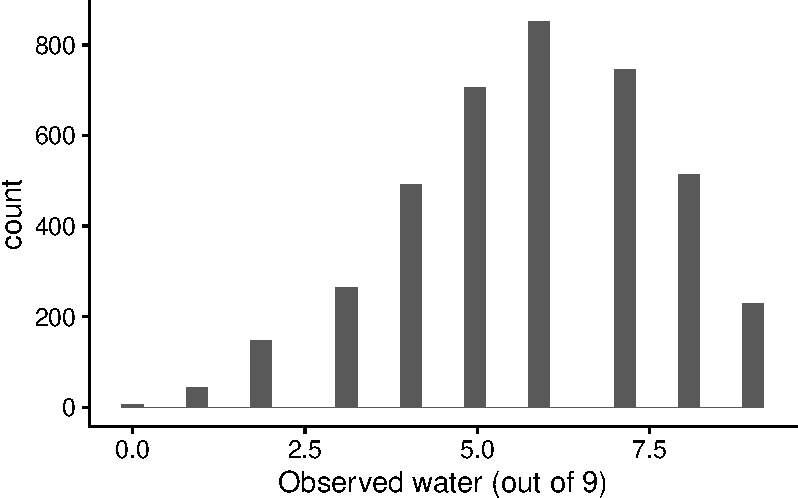
\includegraphics[width=17.1875in,height=\textheight]{lecture02-1_files/figure-pdf/unnamed-chunk-8-1.pdf}

\begin{center}\rule{0.5\linewidth}{0.5pt}\end{center}

\subsubsection{\texorpdfstring{Sampling parameters from the
\textbf{prior}}{Sampling parameters from the prior}}\label{sampling-parameters-from-the-prior}

Oops, we've jumped ahead of ourselves! Best practice is to simulate
values from your prior \textbf{first} and check to see if those priors
are reasonable.

\begin{Shaded}
\begin{Highlighting}[numbers=left,,]
\NormalTok{m1p }\OtherTok{\textless{}{-}}
  \FunctionTok{brm}\NormalTok{(}\AttributeTok{data =} \FunctionTok{list}\NormalTok{(}\AttributeTok{w =} \DecValTok{6}\NormalTok{),                            }
      \AttributeTok{family =} \FunctionTok{binomial}\NormalTok{(}\AttributeTok{link =} \StringTok{"identity"}\NormalTok{),          }
\NormalTok{      w }\SpecialCharTok{|} \FunctionTok{trials}\NormalTok{(}\DecValTok{9}\NormalTok{) }\SpecialCharTok{\textasciitilde{}} \DecValTok{0} \SpecialCharTok{+}\NormalTok{ Intercept,                 }
      \FunctionTok{prior}\NormalTok{(}\FunctionTok{beta}\NormalTok{(}\DecValTok{1}\NormalTok{, }\DecValTok{1}\NormalTok{), }\AttributeTok{class =}\NormalTok{ b, }\AttributeTok{lb =} \DecValTok{0}\NormalTok{, }\AttributeTok{ub =} \DecValTok{1}\NormalTok{),  }
      \AttributeTok{iter =} \DecValTok{5000}\NormalTok{, }\AttributeTok{warmup =} \DecValTok{1000}\NormalTok{, }\AttributeTok{seed =} \DecValTok{3}\NormalTok{, }\AttributeTok{chains=}\DecValTok{1}\NormalTok{,          }
      \AttributeTok{sample\_prior =} \StringTok{"only"}\NormalTok{)}
\end{Highlighting}
\end{Shaded}

\begin{Shaded}
\begin{Highlighting}[]
\NormalTok{samples\_from\_prior }\OtherTok{=} \FunctionTok{as\_draws\_df}\NormalTok{(m1p)}
\NormalTok{samples\_from\_prior }\SpecialCharTok{\%\textgreater{}\%} 
  \FunctionTok{ggplot}\NormalTok{(}\FunctionTok{aes}\NormalTok{(}\AttributeTok{x=}\NormalTok{b\_Intercept)) }\SpecialCharTok{+}
  \FunctionTok{geom\_density}\NormalTok{(}\AttributeTok{fill =} \StringTok{"grey"}\NormalTok{, }\AttributeTok{color =} \StringTok{"white"}\NormalTok{) }\SpecialCharTok{+}
  \FunctionTok{labs}\NormalTok{(}\AttributeTok{x=}\StringTok{"Proportion water"}\NormalTok{, }\AttributeTok{title=}\StringTok{"Prior"}\NormalTok{)}
\end{Highlighting}
\end{Shaded}

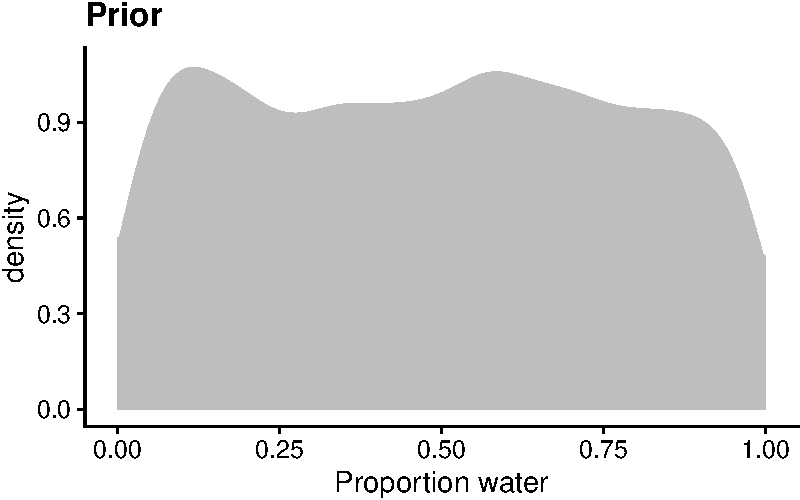
\includegraphics[width=17.1875in,height=\textheight]{lecture02-1_files/figure-pdf/unnamed-chunk-10-1.pdf}

\begin{center}\rule{0.5\linewidth}{0.5pt}\end{center}

\subsubsection{Simulating observations from the
prior}\label{simulating-observations-from-the-prior}

We may also want the \textbf{PRIOR PREDICTIVE DISTRIBUTION} which is the
expected observiations given our prior.

\begin{Shaded}
\begin{Highlighting}[]
\NormalTok{prior\_pd }\OtherTok{=} \FunctionTok{posterior\_predict}\NormalTok{(m1p)}
\FunctionTok{data.frame}\NormalTok{(}\AttributeTok{obs =}\NormalTok{ prior\_pd) }\SpecialCharTok{\%\textgreater{}\%} 
  \FunctionTok{ggplot}\NormalTok{(}\FunctionTok{aes}\NormalTok{(}\AttributeTok{x=}\NormalTok{obs)) }\SpecialCharTok{+}
  \FunctionTok{geom\_histogram}\NormalTok{() }\SpecialCharTok{+}
  \FunctionTok{labs}\NormalTok{(}\AttributeTok{x=}\StringTok{"Observed water (out of 9)"}\NormalTok{)}
\end{Highlighting}
\end{Shaded}

\begin{verbatim}
`stat_bin()` using `bins = 30`. Pick better value with `binwidth`.
\end{verbatim}

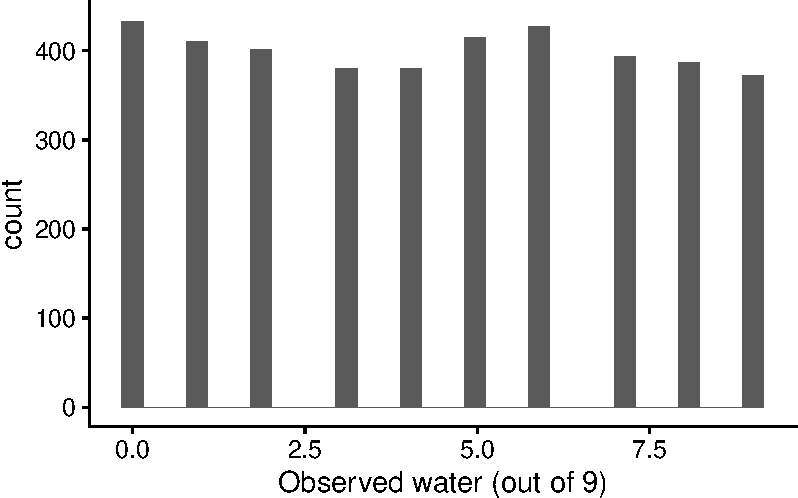
\includegraphics[width=17.1875in,height=\textheight]{lecture02-1_files/figure-pdf/unnamed-chunk-11-1.pdf}

Simulating from your priors -- \textbf{prior predictive simulation} --
is an essential part of modeling. This allows you to see what your
choices imply about the data. You'll be able to diagnose bad choices.

\begin{center}\rule{0.5\linewidth}{0.5pt}\end{center}

\subsubsection{an aside about learning in
R}\label{an-aside-about-learning-in-r}

At this point in the course, I'm going to start throwing a lot of code
at you. Do I expect you to memorize this code? Of course not.

Do you need to understand every single thing that's happening in the
code? Nope.

But, you'll learn a lot by taking the time to figure out what's
happening in a code chunk. Class time will frequently include exercises
where I ask you to adapt code I've shared in the slides to a new dataset
or to answer a new problem. When doing so, go back through the old code
and figure out what's going on. Run the code one line at a time. Always
observe the output and take some time to look at the object that was
created or modified. Here are some functions that will be extremely
useful:

\begin{Shaded}
\begin{Highlighting}[]
\FunctionTok{str}\NormalTok{() }\CommentTok{\# what kind of object is this? what is its structure?}
\FunctionTok{dim}\NormalTok{() }\CommentTok{\# what are the dimensions (rows/columns) of this object}
\FunctionTok{head}\NormalTok{() }\CommentTok{\# give me the first bit of this object}
\end{Highlighting}
\end{Shaded}

\begin{Shaded}
\begin{Highlighting}[]
\FunctionTok{str}\NormalTok{(prior\_pd)}
\end{Highlighting}
\end{Shaded}

\begin{verbatim}
 int [1:4000, 1] 6 2 0 1 7 8 0 5 4 4 ...
 - attr(*, "dimnames")=List of 2
  ..$ : NULL
  ..$ : NULL
\end{verbatim}

\begin{Shaded}
\begin{Highlighting}[]
\FunctionTok{dim}\NormalTok{(prior\_pd)}
\end{Highlighting}
\end{Shaded}

\begin{verbatim}
[1] 4000    1
\end{verbatim}

\begin{Shaded}
\begin{Highlighting}[]
\FunctionTok{head}\NormalTok{(prior\_pd)}
\end{Highlighting}
\end{Shaded}

\begin{verbatim}
     [,1]
[1,]    6
[2,]    2
[3,]    0
[4,]    1
[5,]    7
[6,]    8
\end{verbatim}

\begin{center}\rule{0.5\linewidth}{0.5pt}\end{center}

\subsubsection{Continous outcomes}\label{continous-outcomes}

The globe tossing example is cute and easy to work with, but let's move
towards the kinds of variables we more frequently work with. Let's
create a model for some outcome, \(y\) that is continuous.

\begin{align*}
y_i &\sim \text{Normal}(\mu, \sigma) \\
\mu &\sim \text{Normal}(0, 10) \\
\sigma &\sim \text{Uniform}(0, 5)
\end{align*}

\begin{Shaded}
\begin{Highlighting}[]
\FunctionTok{set.seed}\NormalTok{(}\DecValTok{9}\NormalTok{)}
\NormalTok{y }\OtherTok{=} \FunctionTok{rnorm}\NormalTok{(}\AttributeTok{n =} \DecValTok{31}\NormalTok{, }\AttributeTok{mean =} \DecValTok{4}\NormalTok{, }\AttributeTok{sd =}\NormalTok{ .}\DecValTok{5}\NormalTok{)}
\NormalTok{m2 }\OtherTok{=} \FunctionTok{brm}\NormalTok{(}
  \AttributeTok{data =} \FunctionTok{list}\NormalTok{(}\AttributeTok{y=}\NormalTok{y),}
  \AttributeTok{family =}\NormalTok{ gaussian,}
\NormalTok{  y }\SpecialCharTok{\textasciitilde{}} \DecValTok{1}\NormalTok{,}
  \AttributeTok{prior =} \FunctionTok{c}\NormalTok{(}\FunctionTok{prior}\NormalTok{( }\FunctionTok{normal}\NormalTok{(}\DecValTok{0}\NormalTok{,}\DecValTok{10}\NormalTok{), }\AttributeTok{class=}\NormalTok{Intercept),}
            \FunctionTok{prior}\NormalTok{( }\FunctionTok{uniform}\NormalTok{(}\DecValTok{0}\NormalTok{,}\DecValTok{5}\NormalTok{), }\AttributeTok{class=}\NormalTok{sigma)),  }
      \AttributeTok{iter =} \DecValTok{5000}\NormalTok{, }\AttributeTok{warmup =} \DecValTok{1000}\NormalTok{, }\AttributeTok{seed =} \DecValTok{3}\NormalTok{, }\AttributeTok{chains=}\DecValTok{1}\NormalTok{,}
  \AttributeTok{file =} \FunctionTok{here}\NormalTok{(}\StringTok{"files/models/m21.2"}\NormalTok{)}
\NormalTok{)}
\end{Highlighting}
\end{Shaded}

\begin{center}\rule{0.5\linewidth}{0.5pt}\end{center}

\subsection{An example: weight and
height}\label{an-example-weight-and-height}

Using the Howell data (don't load the \texttt{rethinking} package
because it can interfere with \texttt{brms}).

\begin{Shaded}
\begin{Highlighting}[]
\FunctionTok{data}\NormalTok{(}\StringTok{"Howell1"}\NormalTok{, }\AttributeTok{package =} \StringTok{"rethinking"}\NormalTok{)}
\NormalTok{d }\OtherTok{\textless{}{-}}\NormalTok{ Howell1}
\FunctionTok{str}\NormalTok{(d)}
\end{Highlighting}
\end{Shaded}

\begin{verbatim}
'data.frame':   544 obs. of  4 variables:
 $ height: num  152 140 137 157 145 ...
 $ weight: num  47.8 36.5 31.9 53 41.3 ...
 $ age   : num  63 63 65 41 51 35 32 27 19 54 ...
 $ male  : int  1 0 0 1 0 1 0 1 0 1 ...
\end{verbatim}

\begin{Shaded}
\begin{Highlighting}[]
\FunctionTok{library}\NormalTok{(measurements)}
\NormalTok{d}\SpecialCharTok{$}\NormalTok{height }\OtherTok{\textless{}{-}} \FunctionTok{conv\_unit}\NormalTok{(d}\SpecialCharTok{$}\NormalTok{height, }\AttributeTok{from =} \StringTok{"cm"}\NormalTok{, }\AttributeTok{to =} \StringTok{"feet"}\NormalTok{)}
\NormalTok{d}\SpecialCharTok{$}\NormalTok{weight }\OtherTok{\textless{}{-}} \FunctionTok{conv\_unit}\NormalTok{(d}\SpecialCharTok{$}\NormalTok{weight, }\AttributeTok{from =} \StringTok{"kg"}\NormalTok{, }\AttributeTok{to =} \StringTok{"lbs"}\NormalTok{)}
\NormalTok{rethinking}\SpecialCharTok{::}\FunctionTok{precis}\NormalTok{(d)}
\end{Highlighting}
\end{Shaded}

\begin{verbatim}
             mean         sd      5.5%    94.5%      histogram
height  4.5362072  0.9055921  2.661042   5.4375      ▁▁▁▁▂▂▇▇▁
weight 78.5079631 32.4502290 20.636856 120.1583 ▁▂▃▂▂▁▁▃▅▇▇▃▂▁
age    29.3443934 20.7468882  1.000000  66.1350      ▇▅▅▃▅▂▂▁▁
male    0.4724265  0.4996986  0.000000   1.0000     ▇▁▁▁▁▁▁▁▁▇
\end{verbatim}

\begin{Shaded}
\begin{Highlighting}[]
\NormalTok{d2 }\OtherTok{\textless{}{-}}\NormalTok{ d[ d}\SpecialCharTok{$}\NormalTok{age }\SpecialCharTok{\textgreater{}=} \DecValTok{18}\NormalTok{, ]}
\end{Highlighting}
\end{Shaded}

\begin{center}\rule{0.5\linewidth}{0.5pt}\end{center}

\subsubsection{exercise}\label{exercise}

Write a mathematical model for the weights in this data set. (Don't
worry about predicting from other variables yet.)

\subsubsection{solution}\label{solution}

\begin{align*}
w &\sim \text{Normal}(\mu, \sigma) \\
\mu &\sim \text{Normal}(130, 20) \\
\sigma &\sim \text{Uniform}(0, 25) \\
\end{align*}

\begin{center}\rule{0.5\linewidth}{0.5pt}\end{center}

\begin{align*}
w &\sim \text{Normal}(\mu, \sigma) \\
\mu &\sim \text{Normal}(130, 20) \\
\sigma &\sim \text{Uniform}(0, 25) \\
\end{align*}

\subsubsection{exercise}\label{exercise-1}

Simulate from your priors (parameters values and prior predictive
values).

\subsubsection{solution}\label{solution-1}

Sample from your priors:

\begin{Shaded}
\begin{Highlighting}[]
\NormalTok{m3p }\OtherTok{=} \FunctionTok{brm}\NormalTok{(}
  \AttributeTok{data =}\NormalTok{ d2,}
  \AttributeTok{family =}\NormalTok{ gaussian,}
\NormalTok{  weight }\SpecialCharTok{\textasciitilde{}} \DecValTok{1}\NormalTok{,}
  \AttributeTok{prior =} \FunctionTok{c}\NormalTok{(}\FunctionTok{prior}\NormalTok{( }\FunctionTok{normal}\NormalTok{(}\DecValTok{130}\NormalTok{,}\DecValTok{20}\NormalTok{), }\AttributeTok{class=}\NormalTok{Intercept),}
            \FunctionTok{prior}\NormalTok{( }\FunctionTok{uniform}\NormalTok{(}\DecValTok{0}\NormalTok{,}\DecValTok{25}\NormalTok{), }\AttributeTok{class=}\NormalTok{sigma, }\AttributeTok{lb=}\DecValTok{0}\NormalTok{, }\AttributeTok{ub=}\DecValTok{25}\NormalTok{)),  }
      \AttributeTok{iter =} \DecValTok{5000}\NormalTok{, }\AttributeTok{warmup =} \DecValTok{1000}\NormalTok{, }\AttributeTok{seed =} \DecValTok{3}\NormalTok{, }\AttributeTok{chains=}\DecValTok{1}\NormalTok{,}
  \AttributeTok{sample\_prior =} \StringTok{"only"}\NormalTok{)}
\end{Highlighting}
\end{Shaded}

\begin{center}\rule{0.5\linewidth}{0.5pt}\end{center}

Sampling parameter estimates for the Intercept.

\begin{Shaded}
\begin{Highlighting}[]
\FunctionTok{pairs}\NormalTok{(m3p)}
\end{Highlighting}
\end{Shaded}

\begin{verbatim}
Warning: Only one chain in 'x'. This plot is more useful with multiple chains.
\end{verbatim}

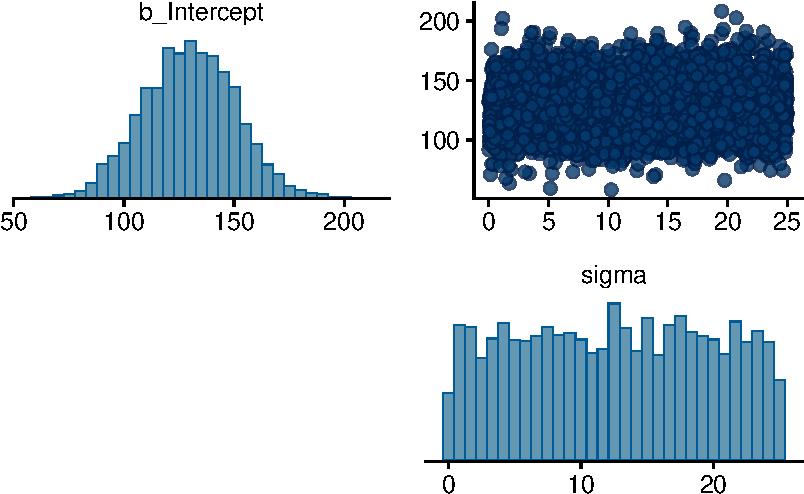
\includegraphics[width=17.1875in,height=\textheight]{lecture02-1_files/figure-pdf/unnamed-chunk-17-1.pdf}

This is a different (shorter) way to plot your posterior. Good things:
it automatically includes the scatterplot so you can see the
implications of how these parameters correlate. Bad things: not
customizable and not useable when you have a lot of parameters.

\begin{center}\rule{0.5\linewidth}{0.5pt}\end{center}

Simulate values of weight.

\begin{Shaded}
\begin{Highlighting}[]
\NormalTok{prior\_pd }\OtherTok{=} \FunctionTok{posterior\_predict}\NormalTok{(m3p)}
\FunctionTok{dim}\NormalTok{(prior\_pd)}
\end{Highlighting}
\end{Shaded}

\begin{verbatim}
[1] 4000  352
\end{verbatim}

\begin{Shaded}
\begin{Highlighting}[]
\FunctionTok{as.data.frame}\NormalTok{(prior\_pd) }\SpecialCharTok{\%\textgreater{}\%} 
  \FunctionTok{pivot\_longer}\NormalTok{(}\FunctionTok{everything}\NormalTok{()) }\SpecialCharTok{\%\textgreater{}\%} 
  \FunctionTok{ggplot}\NormalTok{(}\FunctionTok{aes}\NormalTok{(}\AttributeTok{x=}\NormalTok{value)) }\SpecialCharTok{+}
  \FunctionTok{geom\_histogram}\NormalTok{() }\SpecialCharTok{+}
  \FunctionTok{labs}\NormalTok{(}\AttributeTok{x=}\StringTok{"Expected observed weights (based on prior)"}\NormalTok{)}
\end{Highlighting}
\end{Shaded}

\begin{verbatim}
`stat_bin()` using `bins = 30`. Pick better value with `binwidth`.
\end{verbatim}

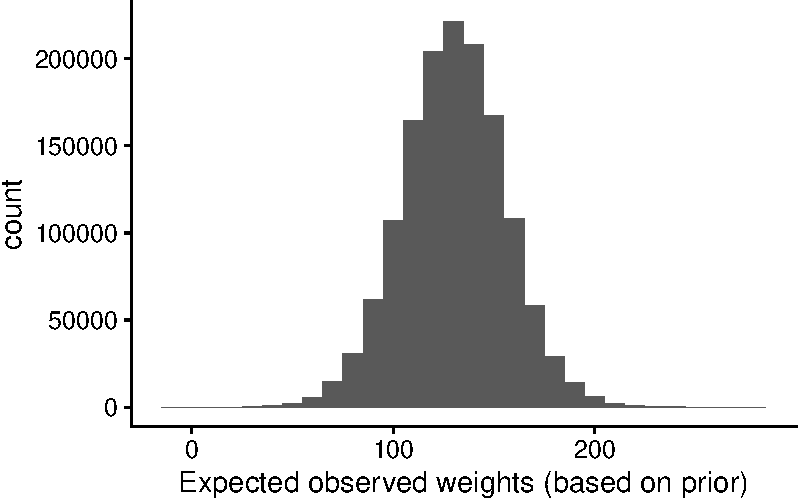
\includegraphics[width=17.1875in,height=\textheight]{lecture02-1_files/figure-pdf/unnamed-chunk-18-1.pdf}

\begin{center}\rule{0.5\linewidth}{0.5pt}\end{center}

Another shorter way:

\begin{Shaded}
\begin{Highlighting}[]
\FunctionTok{pp\_check}\NormalTok{(m3p)}
\end{Highlighting}
\end{Shaded}

\begin{verbatim}
Using 10 posterior draws for ppc type 'dens_overlay' by default.
\end{verbatim}

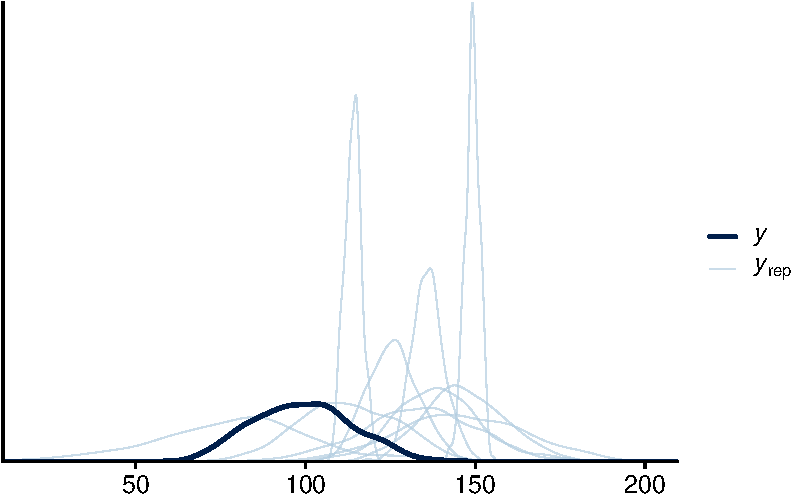
\includegraphics[width=17.1875in,height=\textheight]{lecture02-1_files/figure-pdf/unnamed-chunk-19-1.pdf}

\begin{center}\rule{0.5\linewidth}{0.5pt}\end{center}

\subsubsection{Fit the model}\label{fit-the-model}

\begin{Shaded}
\begin{Highlighting}[]
\NormalTok{m3 }\OtherTok{=} \FunctionTok{brm}\NormalTok{(}
  \AttributeTok{data =}\NormalTok{ d2,}
  \AttributeTok{family =}\NormalTok{ gaussian,}
\NormalTok{  weight }\SpecialCharTok{\textasciitilde{}} \DecValTok{1}\NormalTok{,}
  \AttributeTok{prior =} \FunctionTok{c}\NormalTok{(}\FunctionTok{prior}\NormalTok{( }\FunctionTok{normal}\NormalTok{(}\DecValTok{130}\NormalTok{,}\DecValTok{20}\NormalTok{), }\AttributeTok{class=}\NormalTok{Intercept),}
            \FunctionTok{prior}\NormalTok{( }\FunctionTok{uniform}\NormalTok{(}\DecValTok{0}\NormalTok{,}\DecValTok{25}\NormalTok{), }\AttributeTok{class=}\NormalTok{sigma, }\AttributeTok{lb=}\DecValTok{0}\NormalTok{, }\AttributeTok{ub=}\DecValTok{25}\NormalTok{)),  }
      \AttributeTok{iter =} \DecValTok{5000}\NormalTok{, }\AttributeTok{warmup =} \DecValTok{1000}\NormalTok{, }\AttributeTok{seed =} \DecValTok{3}\NormalTok{, }\AttributeTok{chains=}\DecValTok{1}\NormalTok{,}
  \AttributeTok{file =} \FunctionTok{here}\NormalTok{(}\StringTok{"files/models/m21.3"}\NormalTok{))}
\end{Highlighting}
\end{Shaded}

\begin{Shaded}
\begin{Highlighting}[]
\FunctionTok{posterior\_summary}\NormalTok{(m3)}
\end{Highlighting}
\end{Shaded}

\begin{verbatim}
                Estimate  Est.Error         Q2.5        Q97.5
b_Intercept    99.221909 0.75720356    97.751074   100.737488
sigma          14.291987 0.55198322    13.254363    15.428183
Intercept      99.221909 0.75720356    97.751074   100.737488
lprior         -8.318377 0.05827127    -8.433538    -8.203915
lp__        -1441.294276 1.02695551 -1444.235605 -1440.292326
\end{verbatim}

\begin{center}\rule{0.5\linewidth}{0.5pt}\end{center}

\begin{Shaded}
\begin{Highlighting}[]
\FunctionTok{pairs}\NormalTok{(m3)}
\end{Highlighting}
\end{Shaded}

\begin{verbatim}
Warning: Only one chain in 'x'. This plot is more useful with multiple chains.
\end{verbatim}

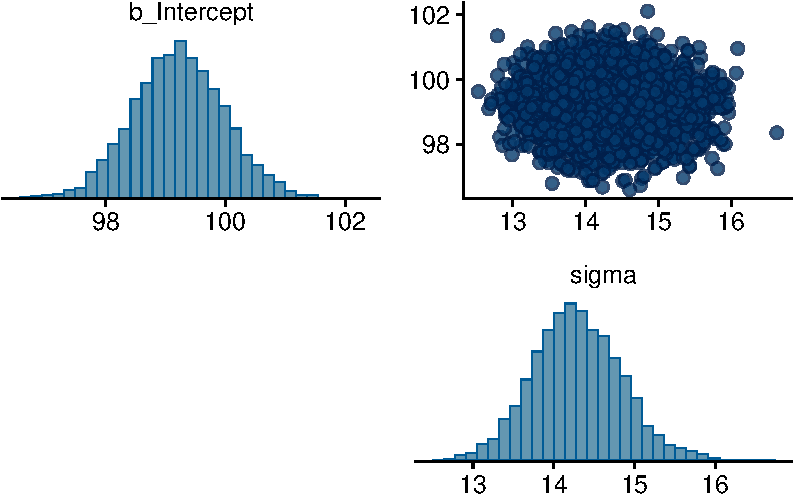
\includegraphics[width=17.1875in,height=\textheight]{lecture02-1_files/figure-pdf/unnamed-chunk-22-1.pdf}

\begin{center}\rule{0.5\linewidth}{0.5pt}\end{center}

\begin{Shaded}
\begin{Highlighting}[]
\FunctionTok{posterior\_predict}\NormalTok{(m3) }\SpecialCharTok{\%\textgreater{}\%} 
  \FunctionTok{as.data.frame}\NormalTok{() }\SpecialCharTok{\%\textgreater{}\%} 
  \FunctionTok{pivot\_longer}\NormalTok{(}\FunctionTok{everything}\NormalTok{()) }\SpecialCharTok{\%\textgreater{}\%} 
  \FunctionTok{ggplot}\NormalTok{(}\FunctionTok{aes}\NormalTok{(}\AttributeTok{x=}\NormalTok{value)) }\SpecialCharTok{+}
  \FunctionTok{geom\_density}\NormalTok{(}\AttributeTok{fill =} \StringTok{"grey"}\NormalTok{, }\AttributeTok{color =} \StringTok{"white"}\NormalTok{) }\SpecialCharTok{+}
  \FunctionTok{geom\_density}\NormalTok{( }\FunctionTok{aes}\NormalTok{(}\AttributeTok{x =}\NormalTok{ weight), }\AttributeTok{data=}\NormalTok{d2, }\AttributeTok{inherit.aes =}\NormalTok{ F) }
\end{Highlighting}
\end{Shaded}

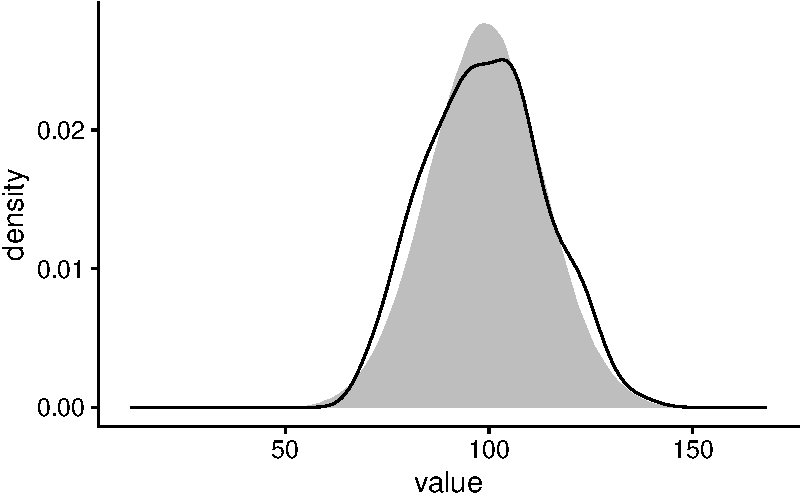
\includegraphics[width=17.1875in,height=\textheight]{lecture02-1_files/figure-pdf/unnamed-chunk-23-1.pdf}

\begin{center}\rule{0.5\linewidth}{0.5pt}\end{center}

\begin{Shaded}
\begin{Highlighting}[]
\FunctionTok{pp\_check}\NormalTok{(m3)}
\end{Highlighting}
\end{Shaded}

\begin{verbatim}
Using 10 posterior draws for ppc type 'dens_overlay' by default.
\end{verbatim}

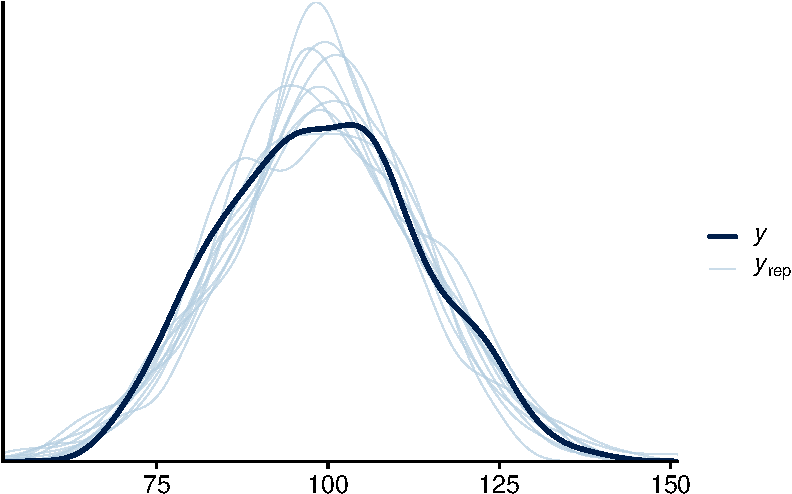
\includegraphics[width=17.1875in,height=\textheight]{lecture02-1_files/figure-pdf/unnamed-chunk-24-1.pdf}

\begin{center}\rule{0.5\linewidth}{0.5pt}\end{center}

\subsection{Adding in a linear
component}\label{adding-in-a-linear-component}

We might assume that height and weight are associated with each other.
Indeed, within our sample:

\begin{Shaded}
\begin{Highlighting}[]
\FunctionTok{plot}\NormalTok{(d2}\SpecialCharTok{$}\NormalTok{weight }\SpecialCharTok{\textasciitilde{}}\NormalTok{ d2}\SpecialCharTok{$}\NormalTok{height)}
\end{Highlighting}
\end{Shaded}

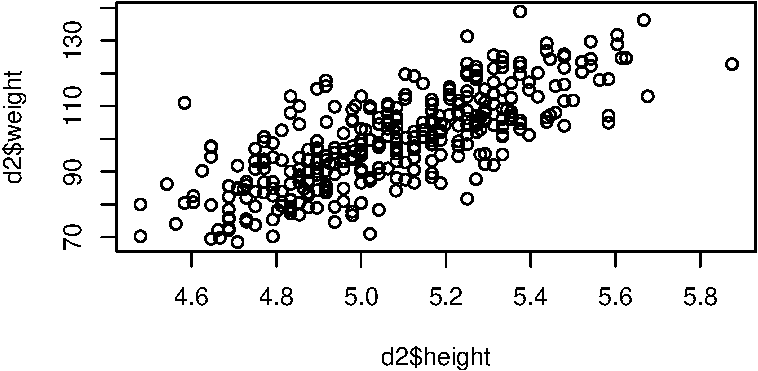
\includegraphics[width=17.1875in,height=\textheight]{lecture02-1_files/figure-pdf/unnamed-chunk-25-1.pdf}

\begin{center}\rule{0.5\linewidth}{0.5pt}\end{center}

\subsubsection{exercise}\label{exercise-2}

Update your mathematical model to incorporate height.

\begin{align*}
w_i &\sim \text{Normal}(\mu_i, \sigma) \\
\mu_i &= \alpha + \beta h_i \\
\alpha &\sim \text{Normal}(??, ??) \\
\beta &\sim \text{Normal}(0, 25) \\
\sigma &\sim \text{Uniform}(0, 25) \\
\end{align*}

\(=\) is deterministic -- once we know other variables, \(\mu_i\) is
known with certainty

made-up parameters are the targets of learning

\begin{center}\rule{0.5\linewidth}{0.5pt}\end{center}

\subsubsection{exercise}\label{exercise-3}

Update your mathematical model to incorporate height.

\begin{align*}
w_i &\sim \text{Normal}(\mu_i, \sigma) \\
\mu_i &= \alpha + \beta (h_i - \bar{h}) \\
\alpha &\sim \text{Normal}(130, 20) \\
\beta &\sim \text{Normal}(0, 25) \\
\sigma &\sim \text{Uniform}(0, 25) \\
\end{align*}

\(=\) is deterministic -- once we know other variables, \(\mu_i\) is
known with certainty

made-up parameters are the targets of learning

\begin{center}\rule{0.5\linewidth}{0.5pt}\end{center}

\begin{align*}
w_i &\sim \text{Normal}(\mu_i, \sigma) \\
\mu_i &= \alpha + \beta (h_i - \bar{h}) \\
\alpha &\sim \text{Normal}(130, 20) \\
\beta &\sim \text{Normal}(0, 25) \\
\sigma &\sim \text{Uniform}(0, 25) \\
\end{align*}

To update our brms code:

\begin{Shaded}
\begin{Highlighting}[]
\NormalTok{d2}\SpecialCharTok{$}\NormalTok{height\_c }\OtherTok{=}\NormalTok{ d2}\SpecialCharTok{$}\NormalTok{height }\SpecialCharTok{{-}} \FunctionTok{mean}\NormalTok{(d2}\SpecialCharTok{$}\NormalTok{height)}
  
\NormalTok{m4p }\OtherTok{=} \FunctionTok{brm}\NormalTok{(}
  \AttributeTok{data =}\NormalTok{ d2,}
  \AttributeTok{family =}\NormalTok{ gaussian,}
\NormalTok{  weight }\SpecialCharTok{\textasciitilde{}} \DecValTok{1} \SpecialCharTok{+}\NormalTok{ height\_c,}
  \AttributeTok{prior =} \FunctionTok{c}\NormalTok{(}\FunctionTok{prior}\NormalTok{( }\FunctionTok{normal}\NormalTok{(}\DecValTok{130}\NormalTok{,}\DecValTok{20}\NormalTok{), }\AttributeTok{class=}\NormalTok{Intercept),}
            \FunctionTok{prior}\NormalTok{( }\FunctionTok{normal}\NormalTok{(}\DecValTok{0}\NormalTok{,}\DecValTok{25}\NormalTok{),   }\AttributeTok{class=}\NormalTok{b),}
            \FunctionTok{prior}\NormalTok{( }\FunctionTok{uniform}\NormalTok{(}\DecValTok{0}\NormalTok{,}\DecValTok{25}\NormalTok{),  }\AttributeTok{class=}\NormalTok{sigma, }\AttributeTok{lb=}\DecValTok{0}\NormalTok{, }\AttributeTok{ub=}\DecValTok{25}\NormalTok{)),  }
      \AttributeTok{iter =} \DecValTok{5000}\NormalTok{, }\AttributeTok{warmup =} \DecValTok{1000}\NormalTok{, }\AttributeTok{seed =} \DecValTok{3}\NormalTok{, }\AttributeTok{chains=}\DecValTok{1}\NormalTok{,}
  \AttributeTok{sample\_prior =} \StringTok{"only"}\NormalTok{)}
\end{Highlighting}
\end{Shaded}

\begin{center}\rule{0.5\linewidth}{0.5pt}\end{center}

\begin{Shaded}
\begin{Highlighting}[]
\FunctionTok{set.seed}\NormalTok{(}\DecValTok{9}\NormalTok{)}
\NormalTok{samples\_from\_prior }\OtherTok{=} \FunctionTok{as\_draws\_df}\NormalTok{(m4p)}
\FunctionTok{str}\NormalTok{(samples\_from\_prior)}
\end{Highlighting}
\end{Shaded}

\begin{verbatim}
draws_df [4,000 x 9] (S3: draws_df/draws/tbl_df/tbl/data.frame)
 $ b_Intercept: num [1:4000] 167 155.6 149.6 88.7 176.4 ...
 $ b_height_c : num [1:4000] -57.9 -57.2 -18.5 52 -47.3 ...
 $ sigma      : num [1:4000] 14.1 11.8 13.3 2.1 21.1 ...
 $ Intercept  : num [1:4000] 167 155.6 149.6 88.7 176.4 ...
 $ lprior     : num [1:4000] -15.7 -14.7 -12 -15.6 -15.8 ...
 $ lp__       : num [1:4000] -13.8 -12.9 -10.2 -14.9 -14.6 ...
 $ .chain     : int [1:4000] 1 1 1 1 1 1 1 1 1 1 ...
 $ .iteration : int [1:4000] 1 2 3 4 5 6 7 8 9 10 ...
 $ .draw      : int [1:4000] 1 2 3 4 5 6 7 8 9 10 ...
\end{verbatim}

\begin{center}\rule{0.5\linewidth}{0.5pt}\end{center}

\begin{Shaded}
\begin{Highlighting}[]
\NormalTok{d2 }\SpecialCharTok{\%\textgreater{}\%} 
  \FunctionTok{ggplot}\NormalTok{(}\FunctionTok{aes}\NormalTok{(}\AttributeTok{x=}\NormalTok{height\_c, }\AttributeTok{y=}\NormalTok{weight)) }\SpecialCharTok{+}
  \FunctionTok{geom\_blank}\NormalTok{() }\SpecialCharTok{+}
  \FunctionTok{geom\_abline}\NormalTok{( }\FunctionTok{aes}\NormalTok{(}\AttributeTok{intercept=}\NormalTok{b\_Intercept, }\AttributeTok{slope=}\NormalTok{b\_height\_c), }
               \AttributeTok{data=}\NormalTok{samples\_from\_prior[}\DecValTok{1}\SpecialCharTok{:}\DecValTok{50}\NormalTok{, ],}
               \AttributeTok{alpha=}\NormalTok{.}\DecValTok{3}\NormalTok{) }\SpecialCharTok{+}
  \FunctionTok{scale\_x\_continuous}\NormalTok{(}\AttributeTok{name =} \StringTok{"height(feet)"}\NormalTok{, }
                     \AttributeTok{breaks=}\FunctionTok{seq}\NormalTok{(}\DecValTok{4}\NormalTok{,}\DecValTok{6}\NormalTok{,}\AttributeTok{by=}\NormalTok{.}\DecValTok{5}\NormalTok{)}\SpecialCharTok{{-}}\FunctionTok{mean}\NormalTok{(d2}\SpecialCharTok{$}\NormalTok{height),}
                     \AttributeTok{labels=}\FunctionTok{seq}\NormalTok{(}\DecValTok{4}\NormalTok{,}\DecValTok{6}\NormalTok{,}\AttributeTok{by=}\NormalTok{.}\DecValTok{5}\NormalTok{))}
\end{Highlighting}
\end{Shaded}

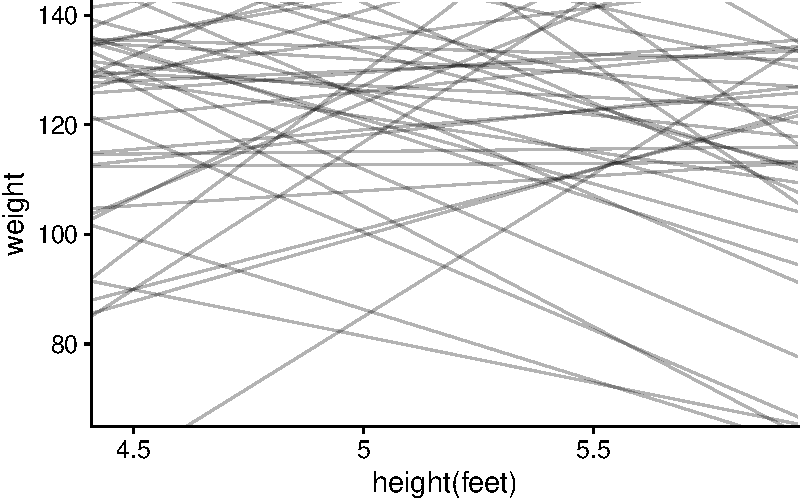
\includegraphics[width=17.1875in,height=\textheight]{lecture02-1_files/figure-pdf/unnamed-chunk-28-1.pdf}

Describe in words what's wrong with our priors.

Slope should not be negative. How can we fix this?

Could use a uniform distribution bounded by 0.

\begin{center}\rule{0.5\linewidth}{0.5pt}\end{center}

\begin{Shaded}
\begin{Highlighting}[]
\NormalTok{m4p }\OtherTok{=} \FunctionTok{brm}\NormalTok{(}
  \AttributeTok{data =}\NormalTok{ d2,}
  \AttributeTok{family =}\NormalTok{ gaussian,}
\NormalTok{  weight }\SpecialCharTok{\textasciitilde{}} \DecValTok{1} \SpecialCharTok{+}\NormalTok{ height\_c,}
  \AttributeTok{prior =} \FunctionTok{c}\NormalTok{(}\FunctionTok{prior}\NormalTok{( }\FunctionTok{normal}\NormalTok{(}\DecValTok{130}\NormalTok{,}\DecValTok{20}\NormalTok{), }\AttributeTok{class=}\NormalTok{Intercept),}
            \FunctionTok{prior}\NormalTok{( }\FunctionTok{uniform}\NormalTok{(}\DecValTok{0}\NormalTok{,}\DecValTok{25}\NormalTok{),   }\AttributeTok{class=}\NormalTok{b),}
            \FunctionTok{prior}\NormalTok{( }\FunctionTok{uniform}\NormalTok{(}\DecValTok{0}\NormalTok{,}\DecValTok{25}\NormalTok{),  }\AttributeTok{class=}\NormalTok{sigma, }\AttributeTok{lb=}\DecValTok{0}\NormalTok{, }\AttributeTok{ub=}\DecValTok{25}\NormalTok{)),  }
      \AttributeTok{iter =} \DecValTok{5000}\NormalTok{, }\AttributeTok{warmup =} \DecValTok{1000}\NormalTok{, }\AttributeTok{seed =} \DecValTok{3}\NormalTok{, }\AttributeTok{chains=}\DecValTok{1}\NormalTok{,}
  \AttributeTok{sample\_prior =} \StringTok{"only"}\NormalTok{)}
\end{Highlighting}
\end{Shaded}

\begin{center}\rule{0.5\linewidth}{0.5pt}\end{center}

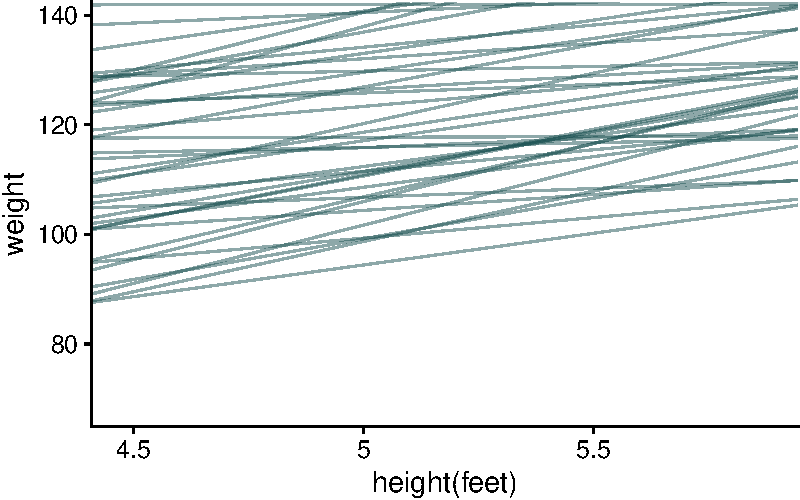
\includegraphics[width=17.1875in,height=\textheight]{lecture02-1_files/figure-pdf/unnamed-chunk-30-1.pdf}

\begin{center}\rule{0.5\linewidth}{0.5pt}\end{center}

\subsubsection{exercise}\label{exercise-4}

Fit the new weight model to the data.

\subsubsection{solution}\label{solution-2}

\begin{Shaded}
\begin{Highlighting}[]
\NormalTok{m4 }\OtherTok{=} \FunctionTok{brm}\NormalTok{(}
  \AttributeTok{data =}\NormalTok{ d2,}
  \AttributeTok{family =}\NormalTok{ gaussian,}
\NormalTok{  weight }\SpecialCharTok{\textasciitilde{}} \DecValTok{1} \SpecialCharTok{+}\NormalTok{ height\_c,}
  \AttributeTok{prior =} \FunctionTok{c}\NormalTok{(}\FunctionTok{prior}\NormalTok{( }\FunctionTok{normal}\NormalTok{(}\DecValTok{130}\NormalTok{,}\DecValTok{20}\NormalTok{), }\AttributeTok{class=}\NormalTok{Intercept),}
            \FunctionTok{prior}\NormalTok{( }\FunctionTok{uniform}\NormalTok{(}\DecValTok{0}\NormalTok{,}\DecValTok{25}\NormalTok{),   }\AttributeTok{class=}\NormalTok{b),}
            \FunctionTok{prior}\NormalTok{( }\FunctionTok{uniform}\NormalTok{(}\DecValTok{0}\NormalTok{,}\DecValTok{25}\NormalTok{),  }\AttributeTok{class=}\NormalTok{sigma, }\AttributeTok{lb=}\DecValTok{0}\NormalTok{, }\AttributeTok{ub=}\DecValTok{25}\NormalTok{)),  }
      \AttributeTok{iter =} \DecValTok{5000}\NormalTok{, }\AttributeTok{warmup =} \DecValTok{1000}\NormalTok{, }\AttributeTok{seed =} \DecValTok{3}\NormalTok{, }\AttributeTok{chains=}\DecValTok{1}\NormalTok{,}
  \AttributeTok{file=}\FunctionTok{here}\NormalTok{(}\StringTok{"files/models/m21.4"}\NormalTok{))}
\FunctionTok{posterior\_summary}\NormalTok{(m4)}
\end{Highlighting}
\end{Shaded}

\begin{verbatim}
               Estimate Est.Error        Q2.5       Q97.5
b_Intercept    99.21508 0.5154139    98.17317   100.20955
b_height_c     24.74661 0.2609169    24.05150    24.99355
sigma          10.36090 0.3898531     9.65234    11.12228
Intercept      99.21508 0.5154139    98.17317   100.20955
lprior        -11.53739 0.0396881   -11.61861   -11.46176
lp__        -1332.15882 1.3936194 -1335.90639 -1330.52002
\end{verbatim}

\begin{center}\rule{0.5\linewidth}{0.5pt}\end{center}

\subsubsection{exercise}\label{exercise-5}

Draw lines from the posterior distribution and plot with the data.

\subsubsection{solution}\label{solution-3}

\begin{Shaded}
\begin{Highlighting}[]
\FunctionTok{set.seed}\NormalTok{(}\DecValTok{9}\NormalTok{)}
\NormalTok{samples\_from\_posterior }\OtherTok{=} \FunctionTok{as\_draws\_df}\NormalTok{(m4)}
\NormalTok{d2}\SpecialCharTok{\%\textgreater{}\%} 
  \FunctionTok{ggplot}\NormalTok{(}\FunctionTok{aes}\NormalTok{(}\AttributeTok{x=}\NormalTok{height\_c, }\AttributeTok{y=}\NormalTok{weight)) }\SpecialCharTok{+}
  \FunctionTok{geom\_point}\NormalTok{(}\AttributeTok{size=}\NormalTok{.}\DecValTok{5}\NormalTok{) }\SpecialCharTok{+}
  \FunctionTok{geom\_abline}\NormalTok{( }\FunctionTok{aes}\NormalTok{(}\AttributeTok{intercept=}\NormalTok{b\_Intercept, }\AttributeTok{slope=}\NormalTok{b\_height\_c), }
               \AttributeTok{data=}\NormalTok{samples\_from\_posterior[}\DecValTok{1}\SpecialCharTok{:}\DecValTok{50}\NormalTok{, ],}
               \AttributeTok{alpha=}\NormalTok{.}\DecValTok{3}\NormalTok{,}
               \AttributeTok{color=}\StringTok{"\#1c5253"}\NormalTok{) }\SpecialCharTok{+}
  \FunctionTok{scale\_x\_continuous}\NormalTok{(}\AttributeTok{name =} \StringTok{"height(feet)"}\NormalTok{, }
                     \AttributeTok{breaks=}\FunctionTok{seq}\NormalTok{(}\DecValTok{4}\NormalTok{,}\DecValTok{6}\NormalTok{,}\AttributeTok{by=}\NormalTok{.}\DecValTok{5}\NormalTok{)}\SpecialCharTok{{-}}\FunctionTok{mean}\NormalTok{(d2}\SpecialCharTok{$}\NormalTok{height),}
                     \AttributeTok{labels=}\FunctionTok{seq}\NormalTok{(}\DecValTok{4}\NormalTok{,}\DecValTok{6}\NormalTok{,}\AttributeTok{by=}\NormalTok{.}\DecValTok{5}\NormalTok{))}
\end{Highlighting}
\end{Shaded}

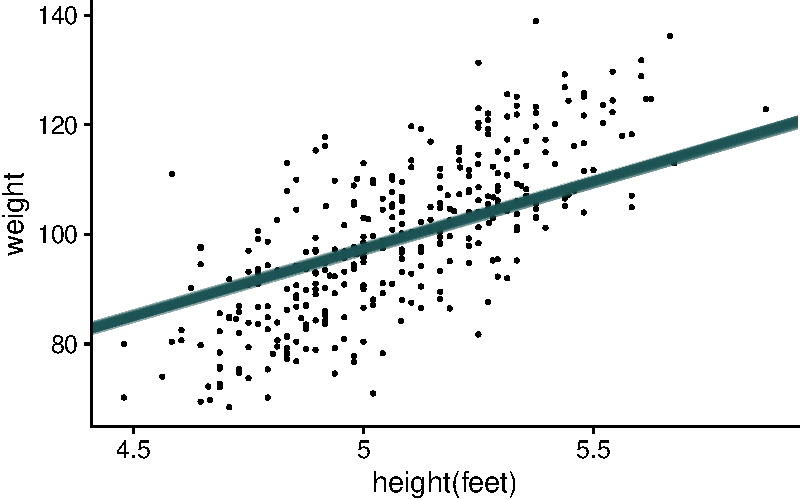
\includegraphics[width=17.1875in,height=\textheight]{lecture02-1_files/figure-pdf/sim-post-1.pdf}

\begin{center}\rule{0.5\linewidth}{0.5pt}\end{center}

A side note: a major concern or critique of Bayesian analysis is that
the subjectivity of the priors allow for nefarious behavior. ``Putting
our thumbs on the scale,'' so to speak. But priors are quickly
overwhelmed by data. Case in point:

\begin{Shaded}
\begin{Highlighting}[numbers=left,,]
\NormalTok{m4e }\OtherTok{=} \FunctionTok{brm}\NormalTok{(}
  \AttributeTok{data =}\NormalTok{ d2,}
  \AttributeTok{family =}\NormalTok{ gaussian,}
\NormalTok{  weight }\SpecialCharTok{\textasciitilde{}} \DecValTok{1} \SpecialCharTok{+}\NormalTok{ height\_c,}
  \AttributeTok{prior =} \FunctionTok{c}\NormalTok{(}\FunctionTok{prior}\NormalTok{( }\FunctionTok{normal}\NormalTok{(}\DecValTok{130}\NormalTok{,}\DecValTok{20}\NormalTok{), }\AttributeTok{class=}\NormalTok{Intercept),}
            \FunctionTok{prior}\NormalTok{( }\FunctionTok{normal}\NormalTok{(}\SpecialCharTok{{-}}\DecValTok{5}\NormalTok{,}\DecValTok{5}\NormalTok{),   }\AttributeTok{class=}\NormalTok{b),}
            \FunctionTok{prior}\NormalTok{( }\FunctionTok{uniform}\NormalTok{(}\DecValTok{0}\NormalTok{,}\DecValTok{25}\NormalTok{),  }\AttributeTok{class=}\NormalTok{sigma, }\AttributeTok{lb=}\DecValTok{0}\NormalTok{, }\AttributeTok{ub=}\DecValTok{25}\NormalTok{)),  }
      \AttributeTok{iter =} \DecValTok{5000}\NormalTok{, }\AttributeTok{warmup =} \DecValTok{1000}\NormalTok{, }\AttributeTok{seed =} \DecValTok{3}\NormalTok{, }\AttributeTok{chains=}\DecValTok{1}\NormalTok{,}
  \AttributeTok{file=}\FunctionTok{here}\NormalTok{(}\StringTok{"files/models/m21.4e"}\NormalTok{))}
\FunctionTok{posterior\_summary}\NormalTok{(m4e)}
\end{Highlighting}
\end{Shaded}

\begin{verbatim}
                Estimate Est.Error         Q2.5       Q97.5
b_Intercept    99.197733 0.5035653    98.214092   100.15932
b_height_c     35.775818 1.8832462    32.177572    39.50070
sigma           9.529429 0.3687178     8.839379    10.27233
Intercept      99.197733 0.5035653    98.214092   100.15932
lprior        -44.172476 3.0738968   -50.456409   -38.49994
lp__        -1334.629214 1.1849503 -1337.645046 -1333.23509
\end{verbatim}

You'll only really get into trouble with uniform priors that have a
boundary, if true population parameter is outside your boundary. A good
rule of thumb is to avoid the uniform distribution. We'll cover other
options for priors for \(\sigma\) in future lectures, but as a preview,
the exponential distribution works very well for this!




\end{document}
